% !TEX root = ../MasterThesis_goto_v1.tex

%%%%%%%%%%%%%%%%%%%%%%%%%%%%%%%%%%%%%%%%%%%%%%%%%%%%%%%%%%%%%%%%%%%%%%%%%%%%%%%%%%%%%%%%%%%%%%%%%%%%%
\chapter{崩壊点検出の為のネットワーク} \label{chap:Networks}

本章では、まず\ref{Net:Data}節で本研究で取り扱うデータの特性について述べる。
また、本研究で扱うデータは全てモンテカルロ (Monte Calro, MC) シミュレーションデータである。
次に、\ref{Net:forVertexFinderwithDL}節にて、どのようにして深層学習を使用した崩壊点検出を実現するかについての発想と作成するネットワークとその役割についての概要的なを説明を行う。
また、使用したコンピュータや深層学習のフレームワークの詳細についてもここで述べる。
作成した個々のネットワークの構造や学習などの詳細や、ネットワーク単体での性能と評価については\ref{Net:PairModel}節、\ref{Net:VertexLSTM}節で解説する。
これらネットワークについては\ref{chap:DeepLearning}章の内容を前提とし、実際に学習に使用する訓練データの詳細や、ハイパーパラメータ・チューニングについてもここで述べる。

%%%%%%%%%%%%%%%%%%%%%%%%%%%%%%%%%%%%%%%%%%%%%%%%%%%%%%%%%%%%%%%%%%%%%%%%%%%%%%%%%%%%%%%%%%%%%%%%%%%%%
\section{データ} \label{Net:Data}

ここでは、本研究で使用したMCシミュレーションデータについて述べる。
特に\ref{Net:Data:DataProperty}項では、データ全体についての性質に関して、\ref{Net:Data:TrackInformationandPreprocessing}項では、本研究で使用する飛跡についての情報と深層学習に使用するための前処理について詳しく述べる。
ただし、各ネットワークの学習に使用する訓練データの詳細に関しては、後の\ref{Net:PM:TrainingandStrategyofPM}や\ref{Net:VLSTM:TrainingandStrategyofVLSTM}で紹介する。

%%%%%%%%%%%%%%%%%%%%%%%%%%%%%%%%%%%%%%%%%%%%%%%%%%%%%%%%%%%%%%%%%%%%%%%%
\subsection{データ全体の性質} \label{Net:Data:DataProperty}

本研究ではWHIZARD\cite{WHIZARDpaper}を用いて生成されたILDフルディテクターシミュレーションデータを使用した。
重心系エネルギーはZ粒子の質量である$91.2 \mathrm{GeV}$、また終状態は、$\rm b\bar{b}$と$\rm c\bar{c}$のデータをそれぞれ用意している。
データ生成において、Beamstrahlung/ISRやビーム偏極は考慮していない。
これらのデータは後述するLCFIPlusでの性能評価\cite{LCFIPluspaper}で使用されたデータと同一のものである。
また、データについて終状態$\rm b\bar{b}$のものは$15$個のサンプルに、終状態$\rm c\bar{c}$のものは$13$個のサンプルに分け使用した。
それぞれの事象数や用途を表\ref{DataSamples}にまとめる。

\begin{table}[htb]
 \centering
 \small
  \begin{tabular}{c c c l} \hline
     データ名 & 事象数 & 飛跡数 & 用途\\ \hline \hline
    $\rm c\bar{c}-01$ & 69581 & 1344465 & データ特性の調査\\ \hline
    $\rm c\bar{c}-02$ & 42204 & 814074 & ネットワークの動作テスト\\ \hline
    $\rm c\bar{c}-03$ & 38662 & 748027 & 飛跡対についてのネットワークの訓練データの作成\\
    $\rm c\bar{c}-04$ & 38712 & 747625 & 飛跡対についてのネットワークの訓練データの作成\\ \hline
    $\rm c\bar{c}-05$ & 38655 & 748089 & 任意の数についてのネットワークの訓練データの作成\\
    $\rm c\bar{c}-06$ & 38645 & 747548 & 任意の数についてのネットワークの訓練データの作成\\ \hline
    $\rm c\bar{c}-07$ & 38643 & 747312 & ネットワークの評価\\
    $\rm c\bar{c}-08$ & 38715 & 748801 & ネットワークの評価\\ \hline 
    $\rm c\bar{c}-09$ & 38705 & 747725 & フレーバータギングの訓練データの作成\\ 
    $\rm c\bar{c}-10$ & 38721 & 748025 & フレーバータギングの訓練データの作成\\
    $\rm c\bar{c}-11$ & 38587 & 747819 & フレーバータギングの訓練データの作成\\ \hline
    $\rm c\bar{c}-12$ & 38723 & 748904 & LCFIPlusとの比較\\
    $\rm c\bar{c}-13$ & 35848 & 693780 & LCFIPlusとの比較\\ \hline\hline
    $\rm b\bar{b}-01$ & 62795 & 1326168 & データ特性の調査\\ \hline
    $\rm b\bar{b}-02$ & 42950 & 909082 & ネットワークの動作テスト\\
    $\rm b\bar{b}-03$ & 34985 & 738105 & ネットワークの動作テスト\\ \hline
    $\rm b\bar{b}-04$ & 34952 & 739130 & 飛跡対についてのネットワークの訓練データの作成\\ 
    $\rm b\bar{b}-05$ & 35047 & 741568 & 飛跡対についてのネットワークの訓練データの作成\\ \hline
    $\rm b\bar{b}-06$ & 35008 & 740662 & 任意の数についてのネットワークの訓練データの作成\\ 
    $\rm b\bar{b}-07$ & 34000 & 718057 & 任意の数についてのネットワークの訓練データの作成\\ \hline
    $\rm b\bar{b}-08$ & 33978 & 717972 & ネットワークの評価\\ 
    $\rm b\bar{b}-09$ & 35008 & 740268 & ネットワークの評価\\ \hline
    $\rm b\bar{b}-10$ & 34954 & 739320 & フレーバータギングの訓練データの作成\\ 
    $\rm b\bar{b}-11$ & 35012 & 740797 & フレーバータギングの訓練データの作成\\ 
    $\rm b\bar{b}-12$ & 34972 & 739953 & フレーバータギングの訓練データの作成\\ \hline
    $\rm b\bar{b}-13$ & 34986 & 739402 & LCFIPlusとの比較\\ 
    $\rm b\bar{b}-14$ & 34910 & 740933 & LCFIPlusとの比較\\ 
    $\rm b\bar{b}-15$ & 10243 & 216499 & LCFIPlusとの比較\\ \hline
  \end{tabular}
  \caption{データサンプルの事象数と用途}
  \label{DataSamples}
\end{table}

データ特性の調査とは本節でのデータそのものについての評価のことである。
また、各訓練データの作成に使用するデータサンプルには、検証データ (Validation data) を含むこととする。
ただし、教師あり学習であるため、学習に使用したデータと評価に使用するデータは完全に分離し、$\rm c\bar{c}-07,08,\ \rm b\bar{b}-08,09$は\ref{Net:PM:PerformanceofPM}項や\ref{Net:VLSTM:PerformanceofVLSTM}項でのみ使用する。
性能の評価において、訓練データを作り直す場合は随時$\rm c\bar{c}-03,04,05,06,\ \rm b\bar{b}-04,05,06,07$のデータサンプルから作成する。
LCFIPlusでのフレーバータギングは\ref{Intro:SoftERILC:JetReconstruction}項で述べた様にBDTが使用されているため、訓練データが必要である。
よって、$\rm c\bar{c}-09,10,11,\ \rm b\bar{b}-10,11,12$はフレーバータギングの訓練データの作成に使用する。
また、全ての訓練データの正解ラベルはMCの真値を使用し作成する。

崩壊点検出を行うにあたって、終状態が$\rm b\bar{b}$の場合は$\rm b \to c$という崩壊過程を辿り、新しいTertiary Vertexが生じることに注意しなければならない。
したがって、終状態が$\rm b\bar{b}$の場合は、このボトム ($\rm b$) ・フレーバーのハドロンによるSecondary Vertexとチャーム ($\rm c$) ・フレーバーのハドロンによるSecondary (Tertiary) Vertexを区別すべきである。
典型的な寿命は光速$c$を用いて、ボトム ($\rm b$) ・フレーバーのハドロンの場合は$c \tau = 400-500 \mathrm{\mu m}$、チャーム ($\rm c$) ・フレーバーのハドロンの場合は$c \tau = 20-300 \mathrm{\mu m}$である。 (図\ref{3-1-1-1FinalStateBB})

\begin{figure}[h]
 \centering
 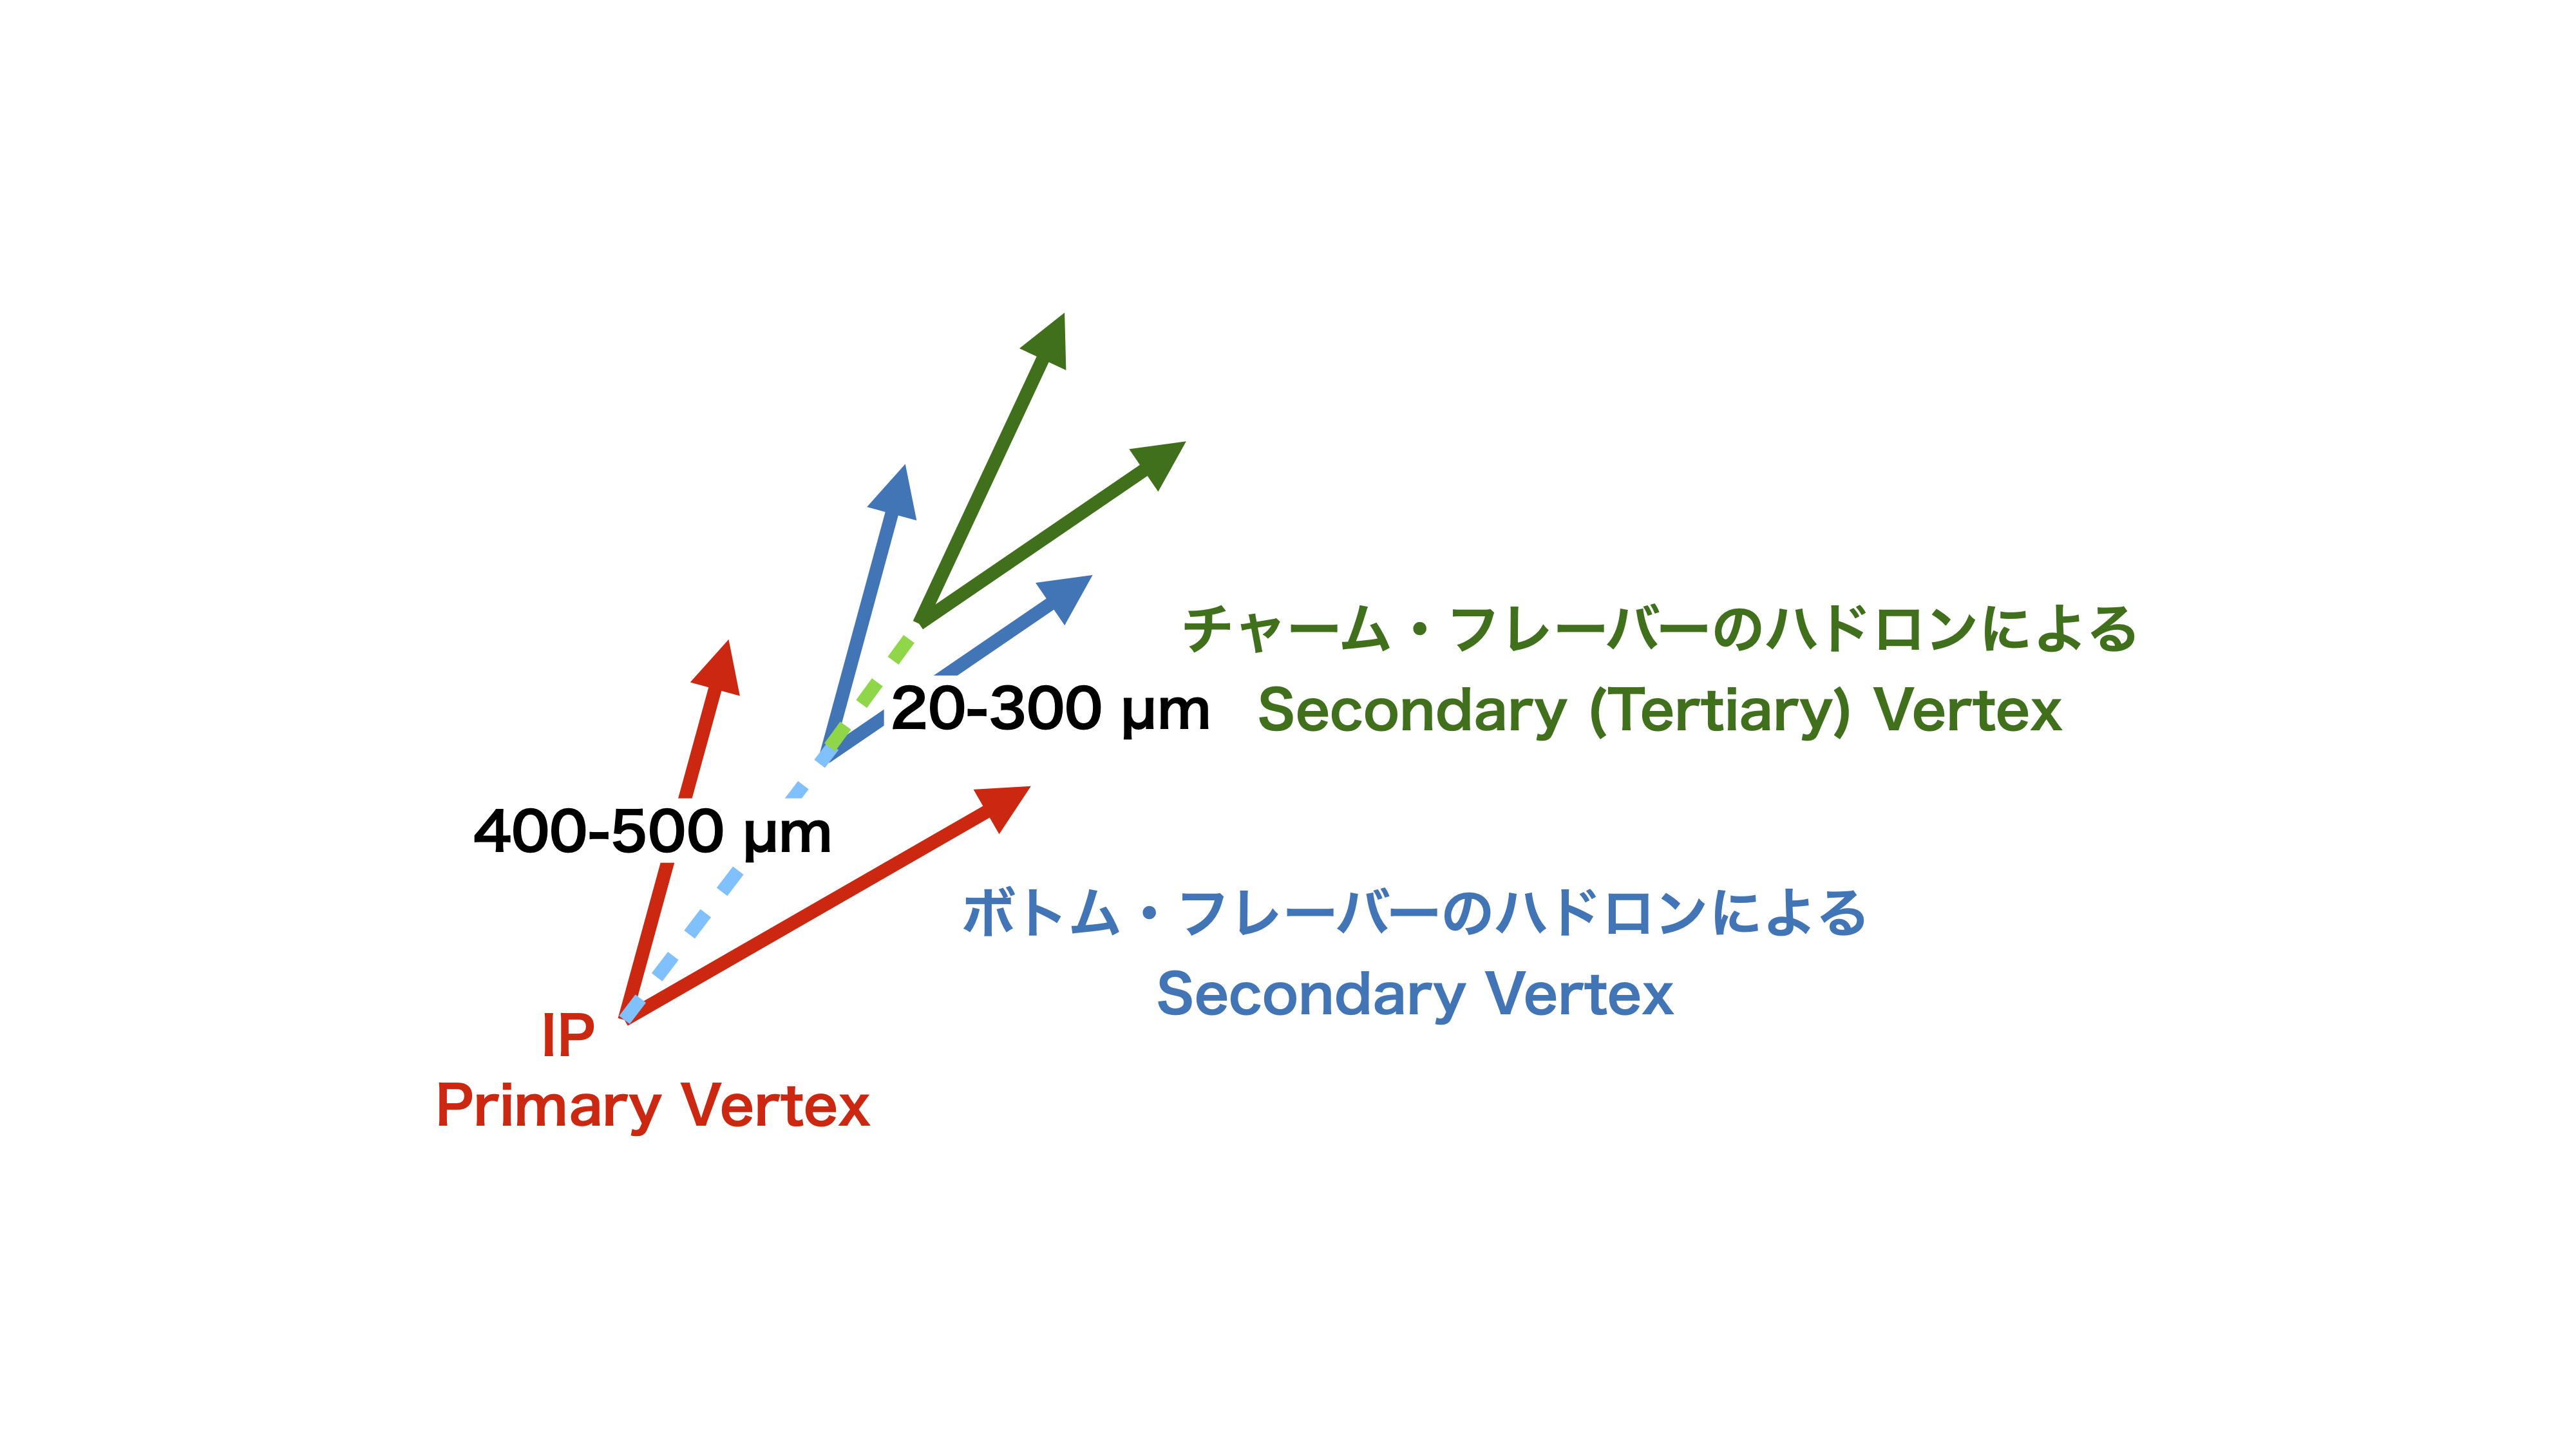
\includegraphics[trim = 0 100 0 50, width=0.9\textwidth]{Figure/3Networks/3-1-1-1FinalStateBB.png}
 \caption{終状態$\rm b\bar{b}$での典型的な崩壊点の例}
 \label{3-1-1-1FinalStateBB}
\end{figure}

図\ref{}は1事象に含まれる飛跡の本数と崩壊点の個数である。

(未完)

%%%%%%%%%%%%%%%%%%%%%%%%%%%%%%%%%%%%%%%%%%%%%%%%%%%%%%%%%%%%%%%%%%%%%%%%
\subsection{飛跡の情報と前処理} \label{Net:Data:TrackInformationandPreprocessing}

本研究では、崩壊点を探索するにあたって飛跡の情報として、図\ref{3-1-1-2TrackParameters}のような位置や運動量を含んだトラック・パラメータ($\rm d_0$, $\rm z_0$, $\rm \phi$, $\rm \Omega$, $\rm \tan{\lambda}$)\cite{TrackParametersLCIO}とその共分散行列、電荷、エネルギーの$22$個の変数を使用した。

\begin{figure}[h]
 \centering
 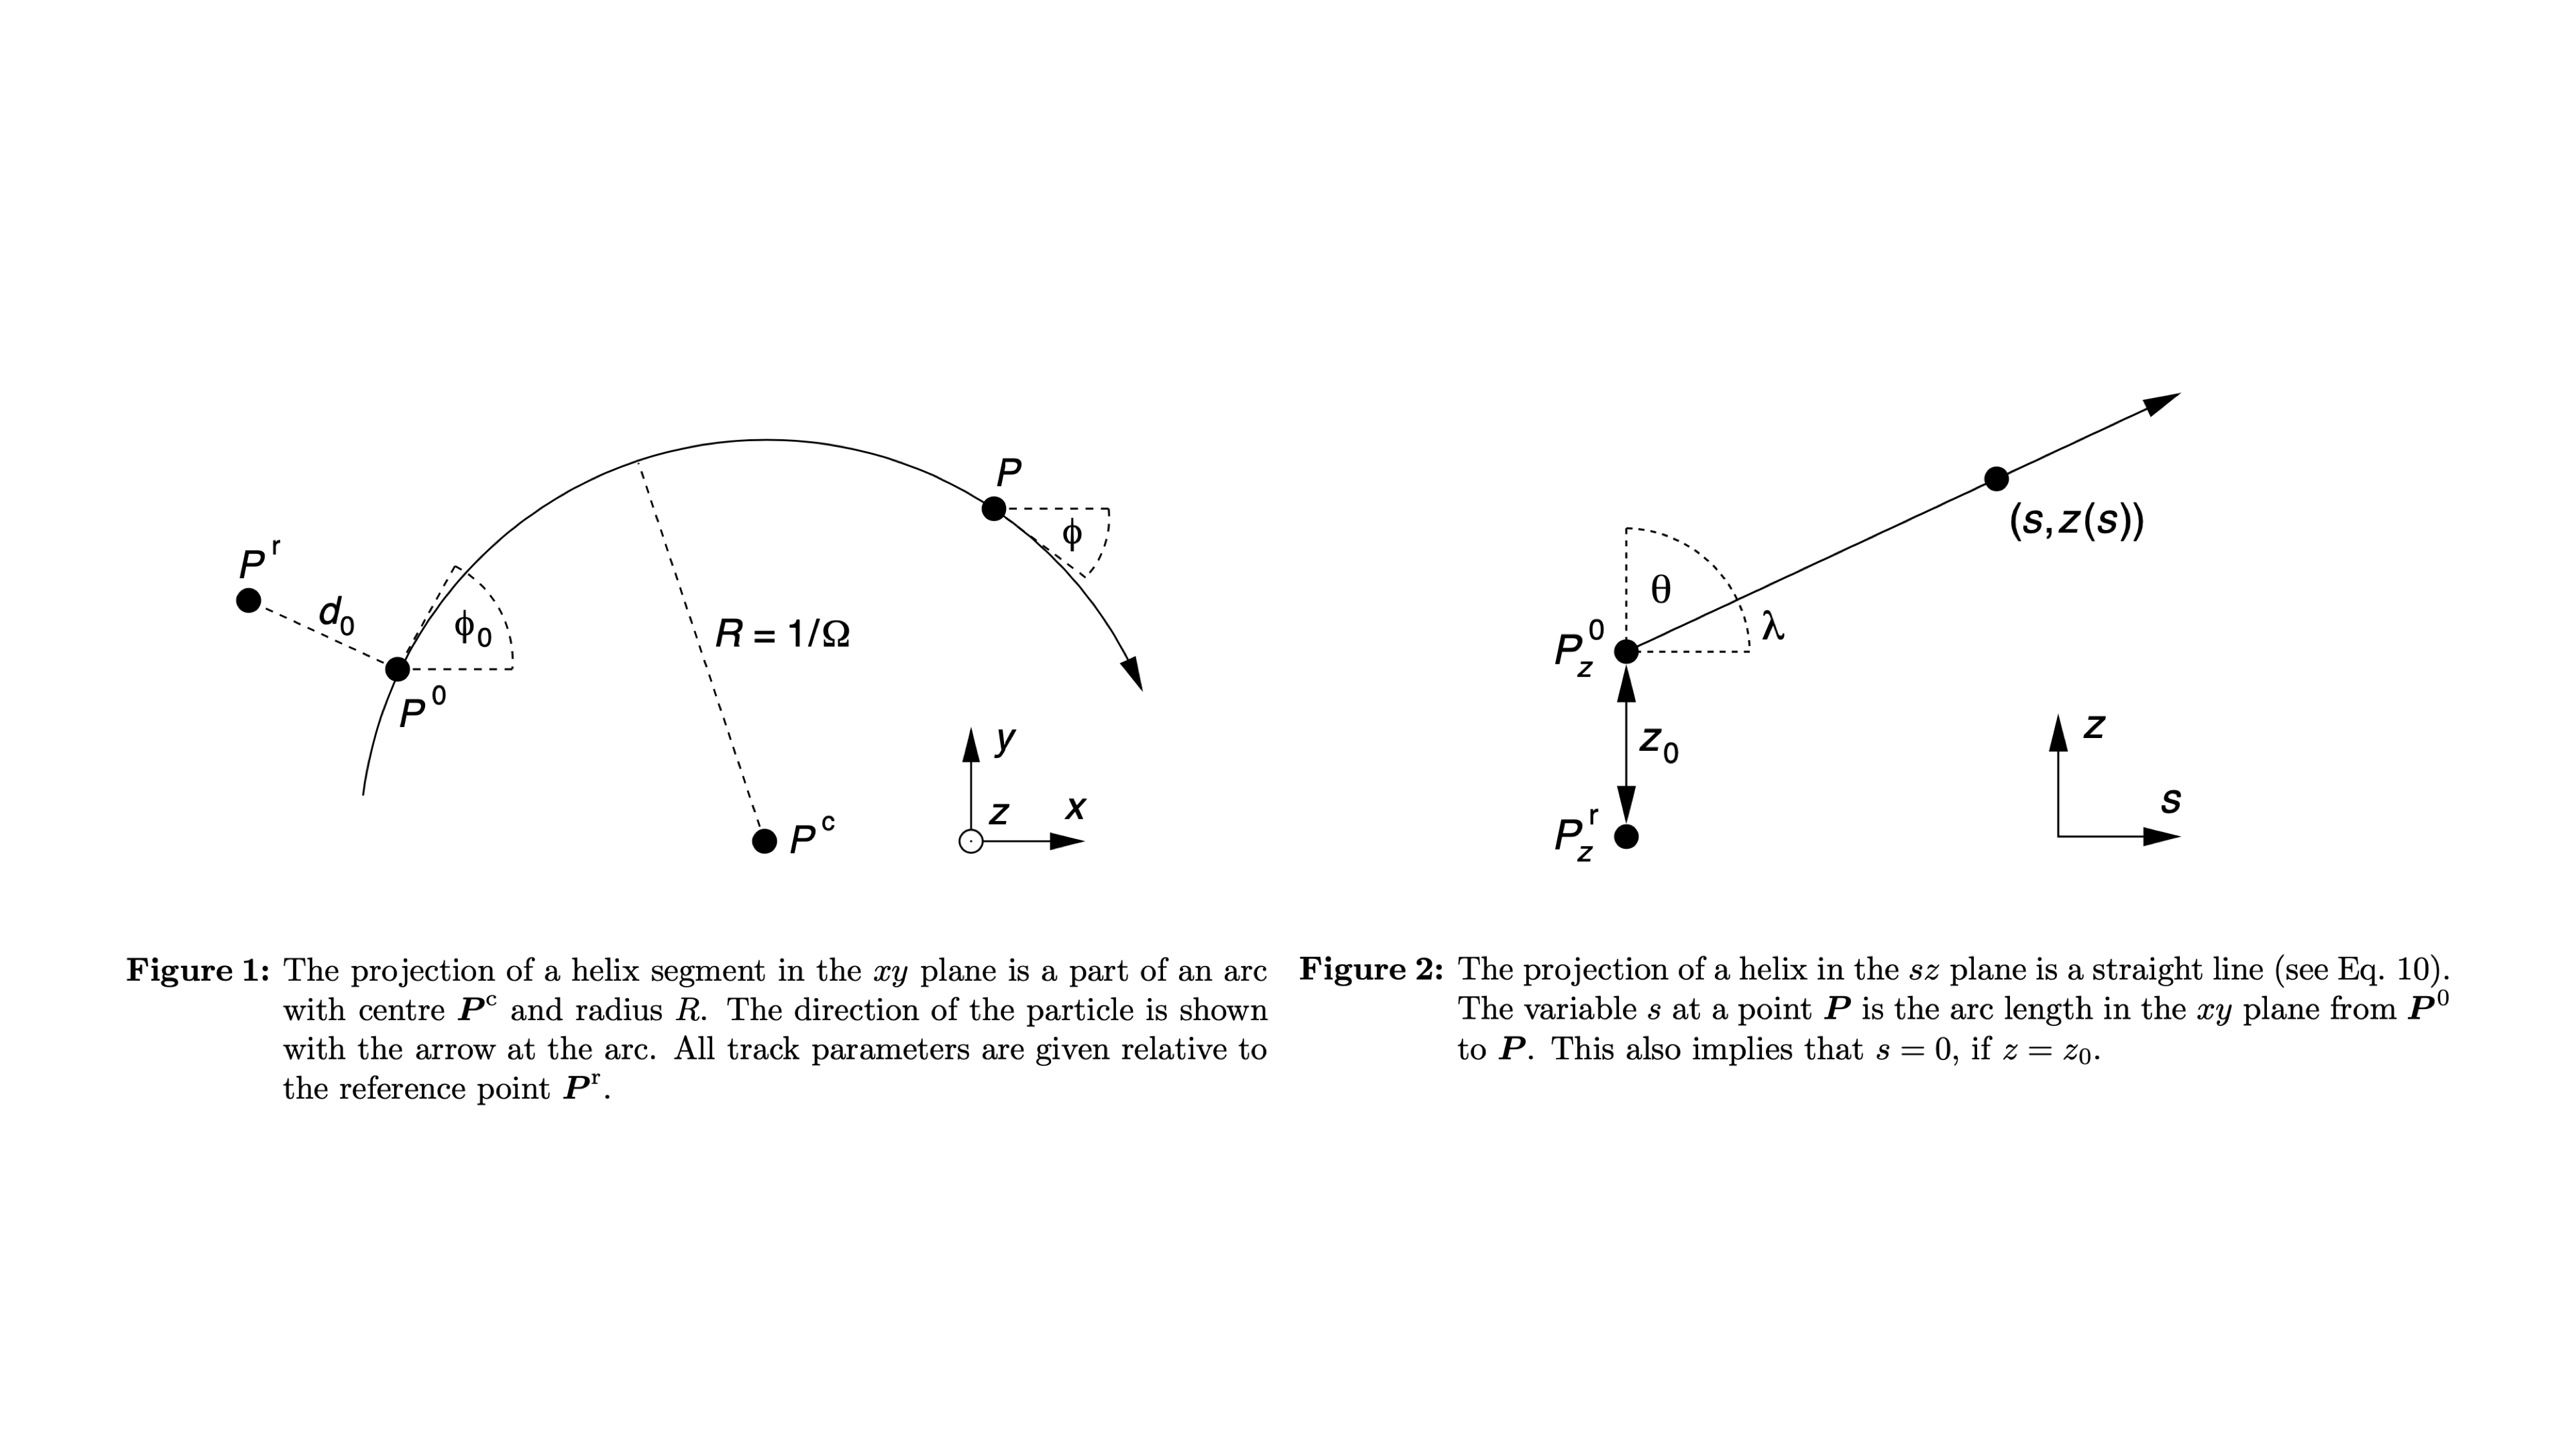
\includegraphics[trim = 0 150 0 150, width=1.0\textwidth]{Figure/3Networks/3-1-1-2TrackParameters.png}
 \caption{トラック・パラメータ\cite{TrackParametersLCIO}}
 \label{3-1-1-2TrackParameters}
\end{figure}

深層学習の入力として扱う場合は、一般に$[-1,\ 1]$の範囲に変数を整形した方が良いと言われている。
したがって、それぞれの変数を以下のような$\tanh$関数や線形関数などを用いて変換した。

\begin{itemize}
 \item トラック・パラメータ\\
 ${\rm d_0} = \tanh{({\rm d_0})}$,
 ${\rm z_0} = \tanh{({\rm z_0})}$,
 ${\rm \phi} = {\rm \phi}/\pi$,
 ${\rm \Omega} = \tanh{(200{\rm \Omega})}$,
 ${\rm \tan{\lambda}} = \tanh{(0.3{\rm d_0})}$
 \item トラック・パラメータの共分散行列 : $\tanh{(8000({\rm x}-0.0005))}$
 \item 電荷 : 変換なし
 \item エネルギー : $\tanh{0.5({\rm x}-5.0)}$
\end{itemize}

トラック・パラメータとエネルギーの変換前の分布と変換後の分布をそれぞれ\ref{3-1-2-1Variables}に示す。

\begin{figure}[h]
 \centering
  %\begin{tabular}{cccc}
  \begin{minipage}{1.0\textwidth}
  \centering
   \begin{minipage}{0.48\textwidth}
    \centering
    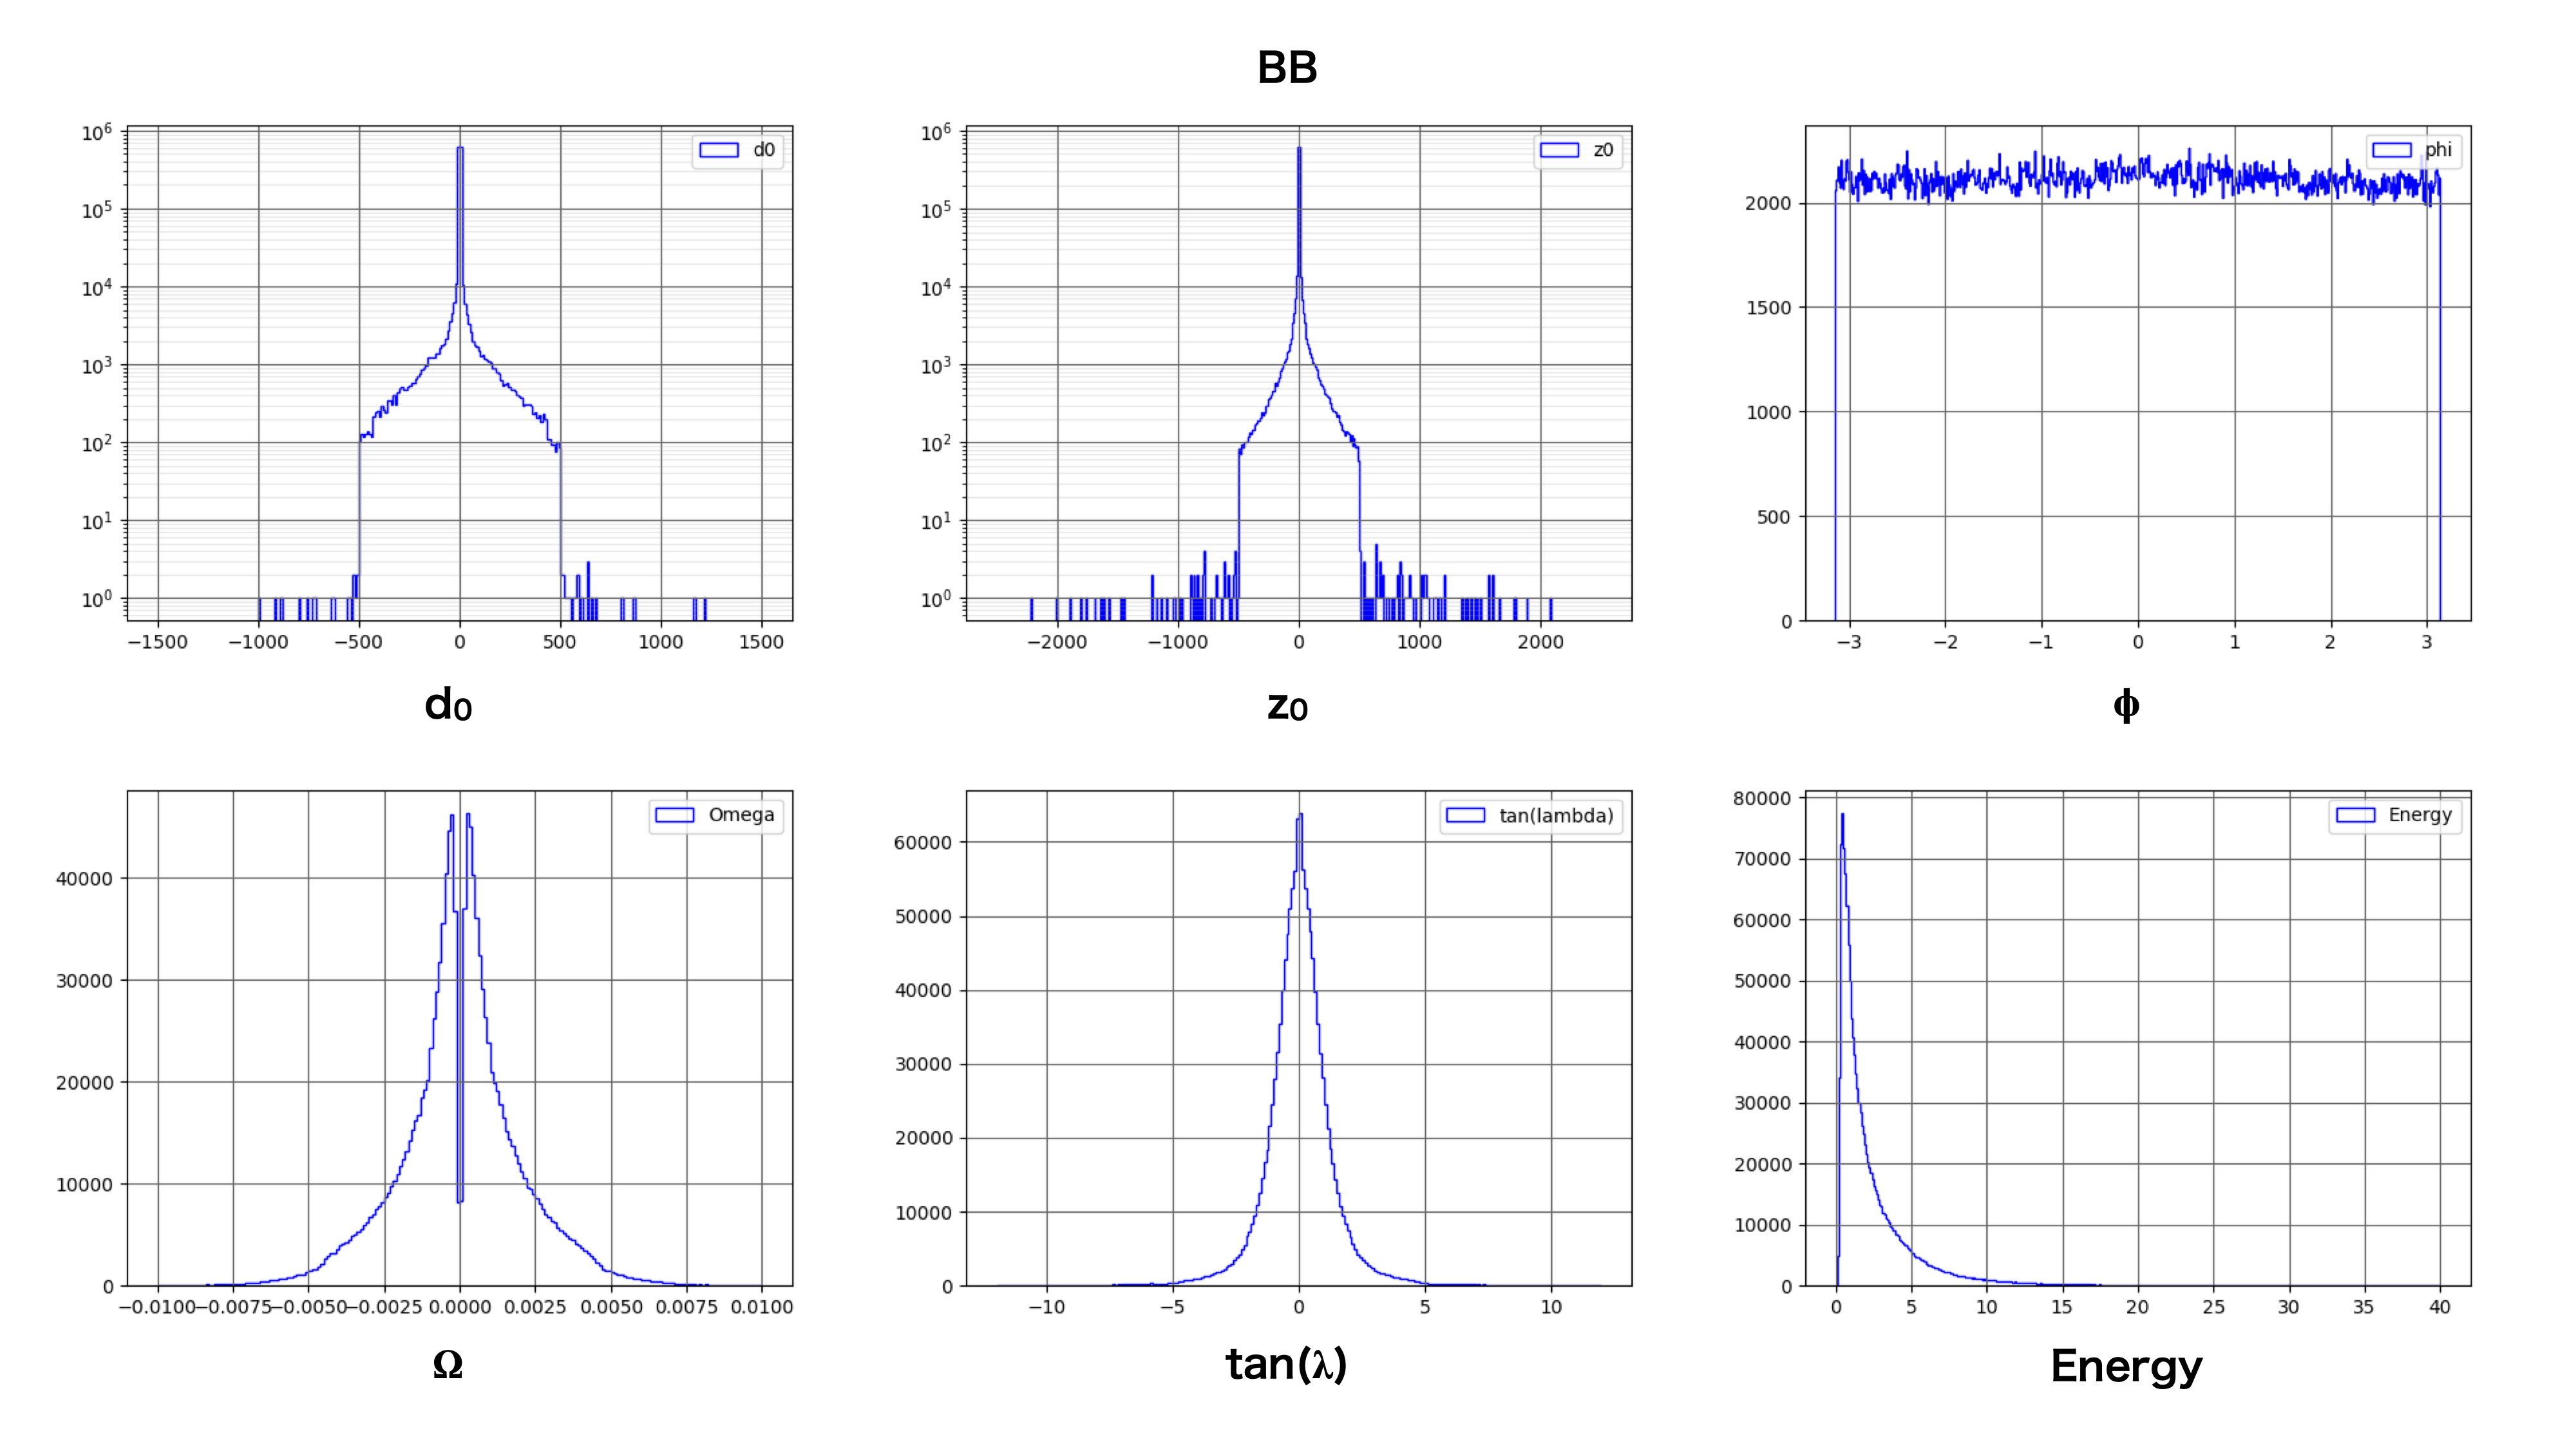
\includegraphics[width=1.0\textwidth, clip]{Figure/3Networks/3-1-2-1OriginalVariablesBB.png}
    \subcaption{終状態$\rm b\bar{b}$での変換前の変数の分布}
    \label{3-1-2-1OriginalVariablesBB}
   \end{minipage}
   \begin{minipage}{0.48\textwidth}
   \centering
    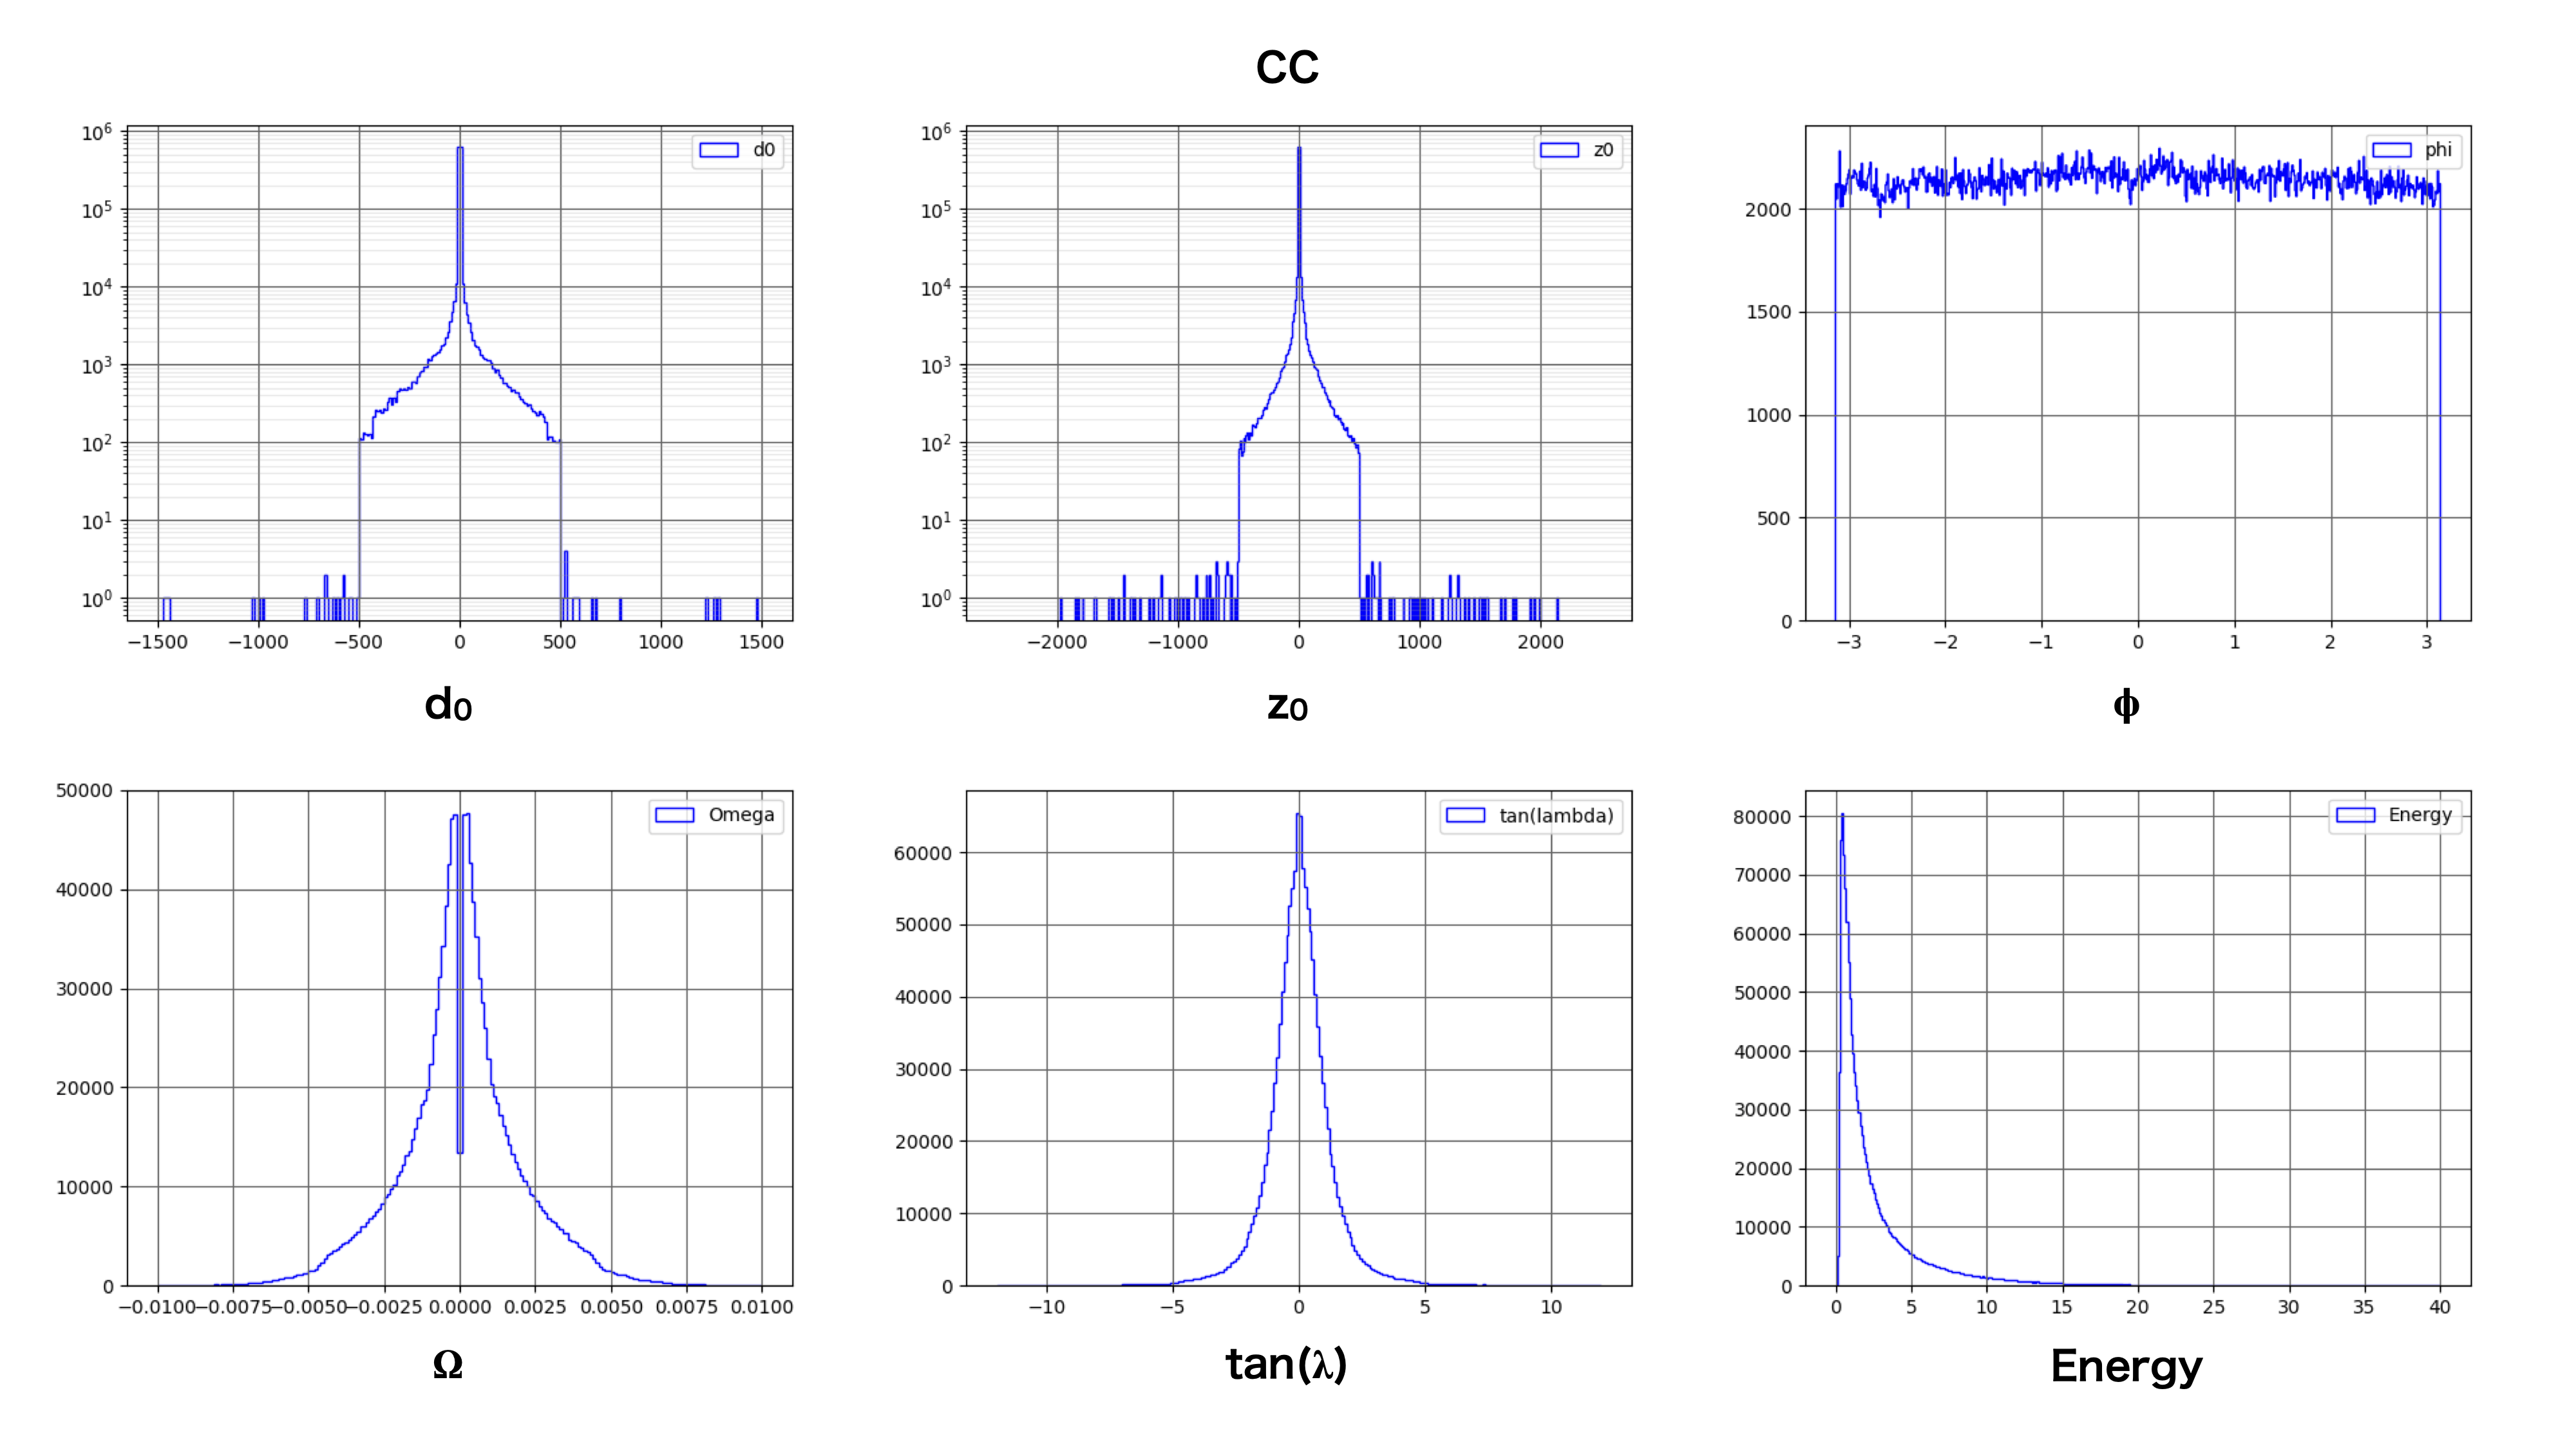
\includegraphics[width=1.0\textwidth, clip]{Figure/3Networks/3-1-2-1OriginalVariablesCC.png}
    \subcaption{終状態$\rm c\bar{c}$での変換前の変数の分布}
    \label{3-1-2-1OriginalVariablesVV}
   \end{minipage}
  \end{minipage}
  
  \begin{minipage}{1.0\textwidth}
  \centering
   \begin{minipage}{0.48\textwidth}
   \centering
    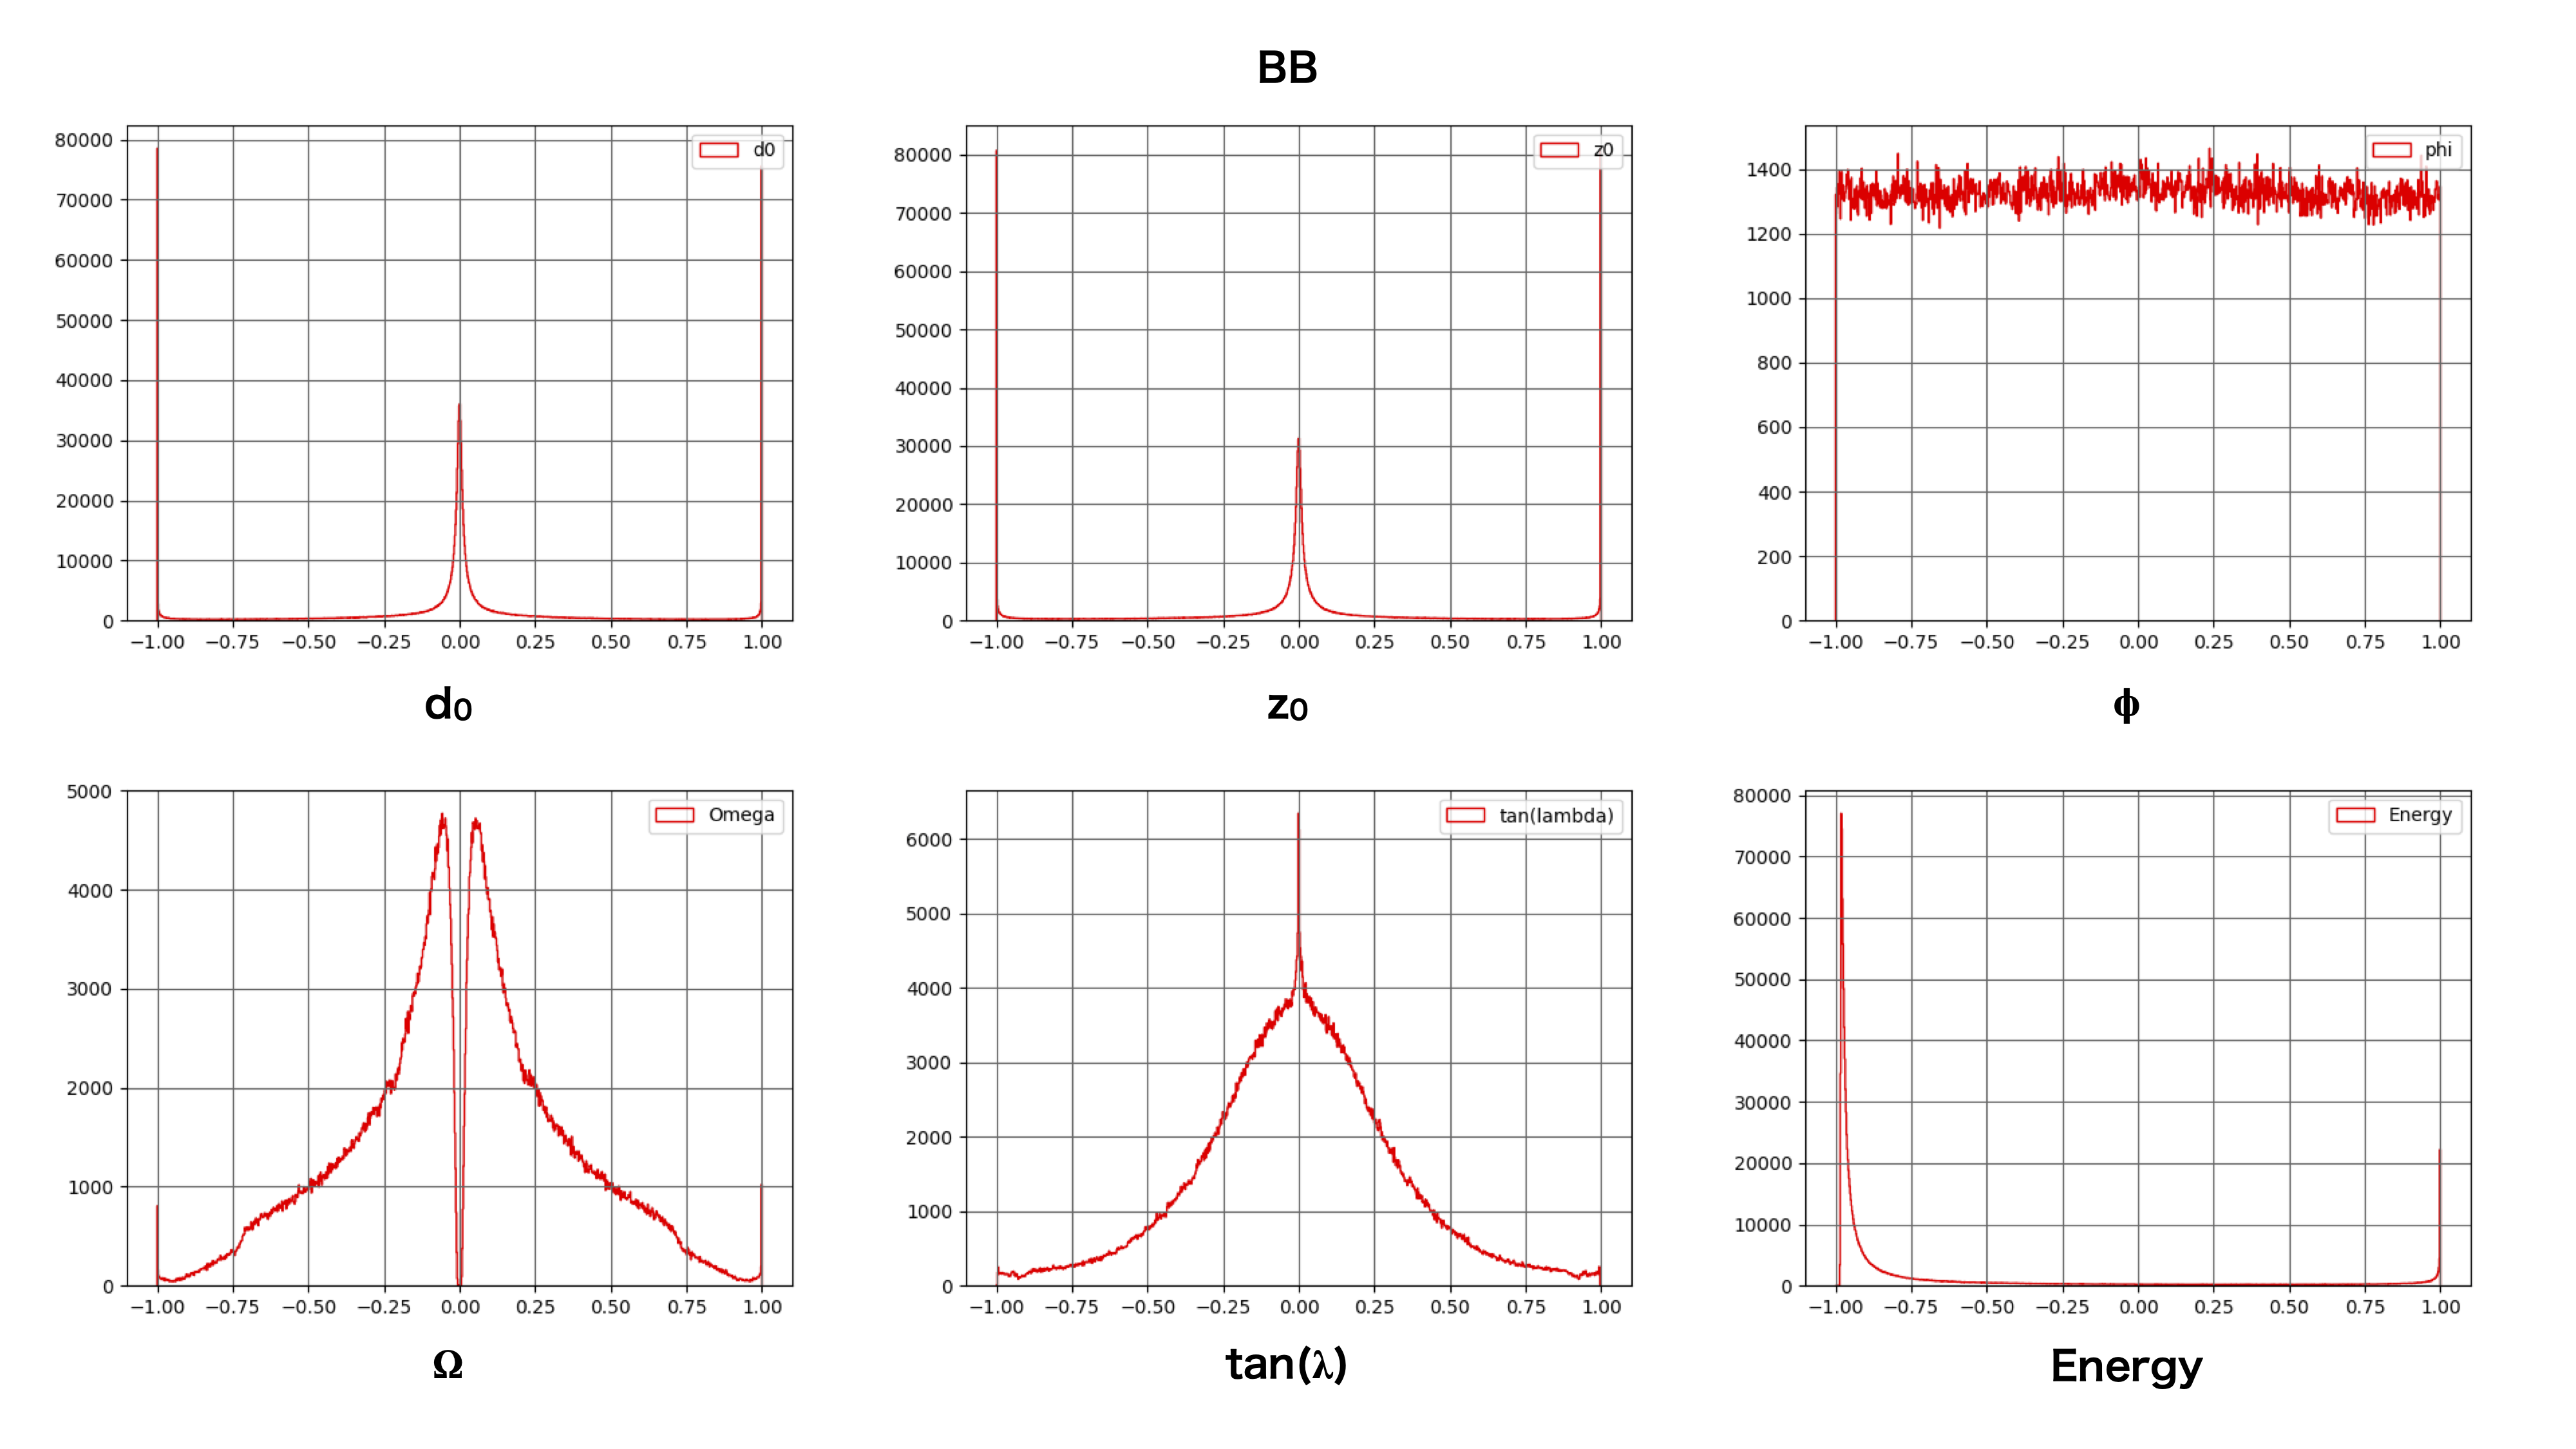
\includegraphics[width=1.0\textwidth, clip]{Figure/3Networks/3-1-2-1ReshapedVariablesBB.png}
    \subcaption{終状態$\rm b\bar{b}$での変換後の変数の分布}
    \label{3-1-2-1ReshapedVariablesBB}
   \end{minipage}
   \begin{minipage}{0.48\textwidth}
   \centering
    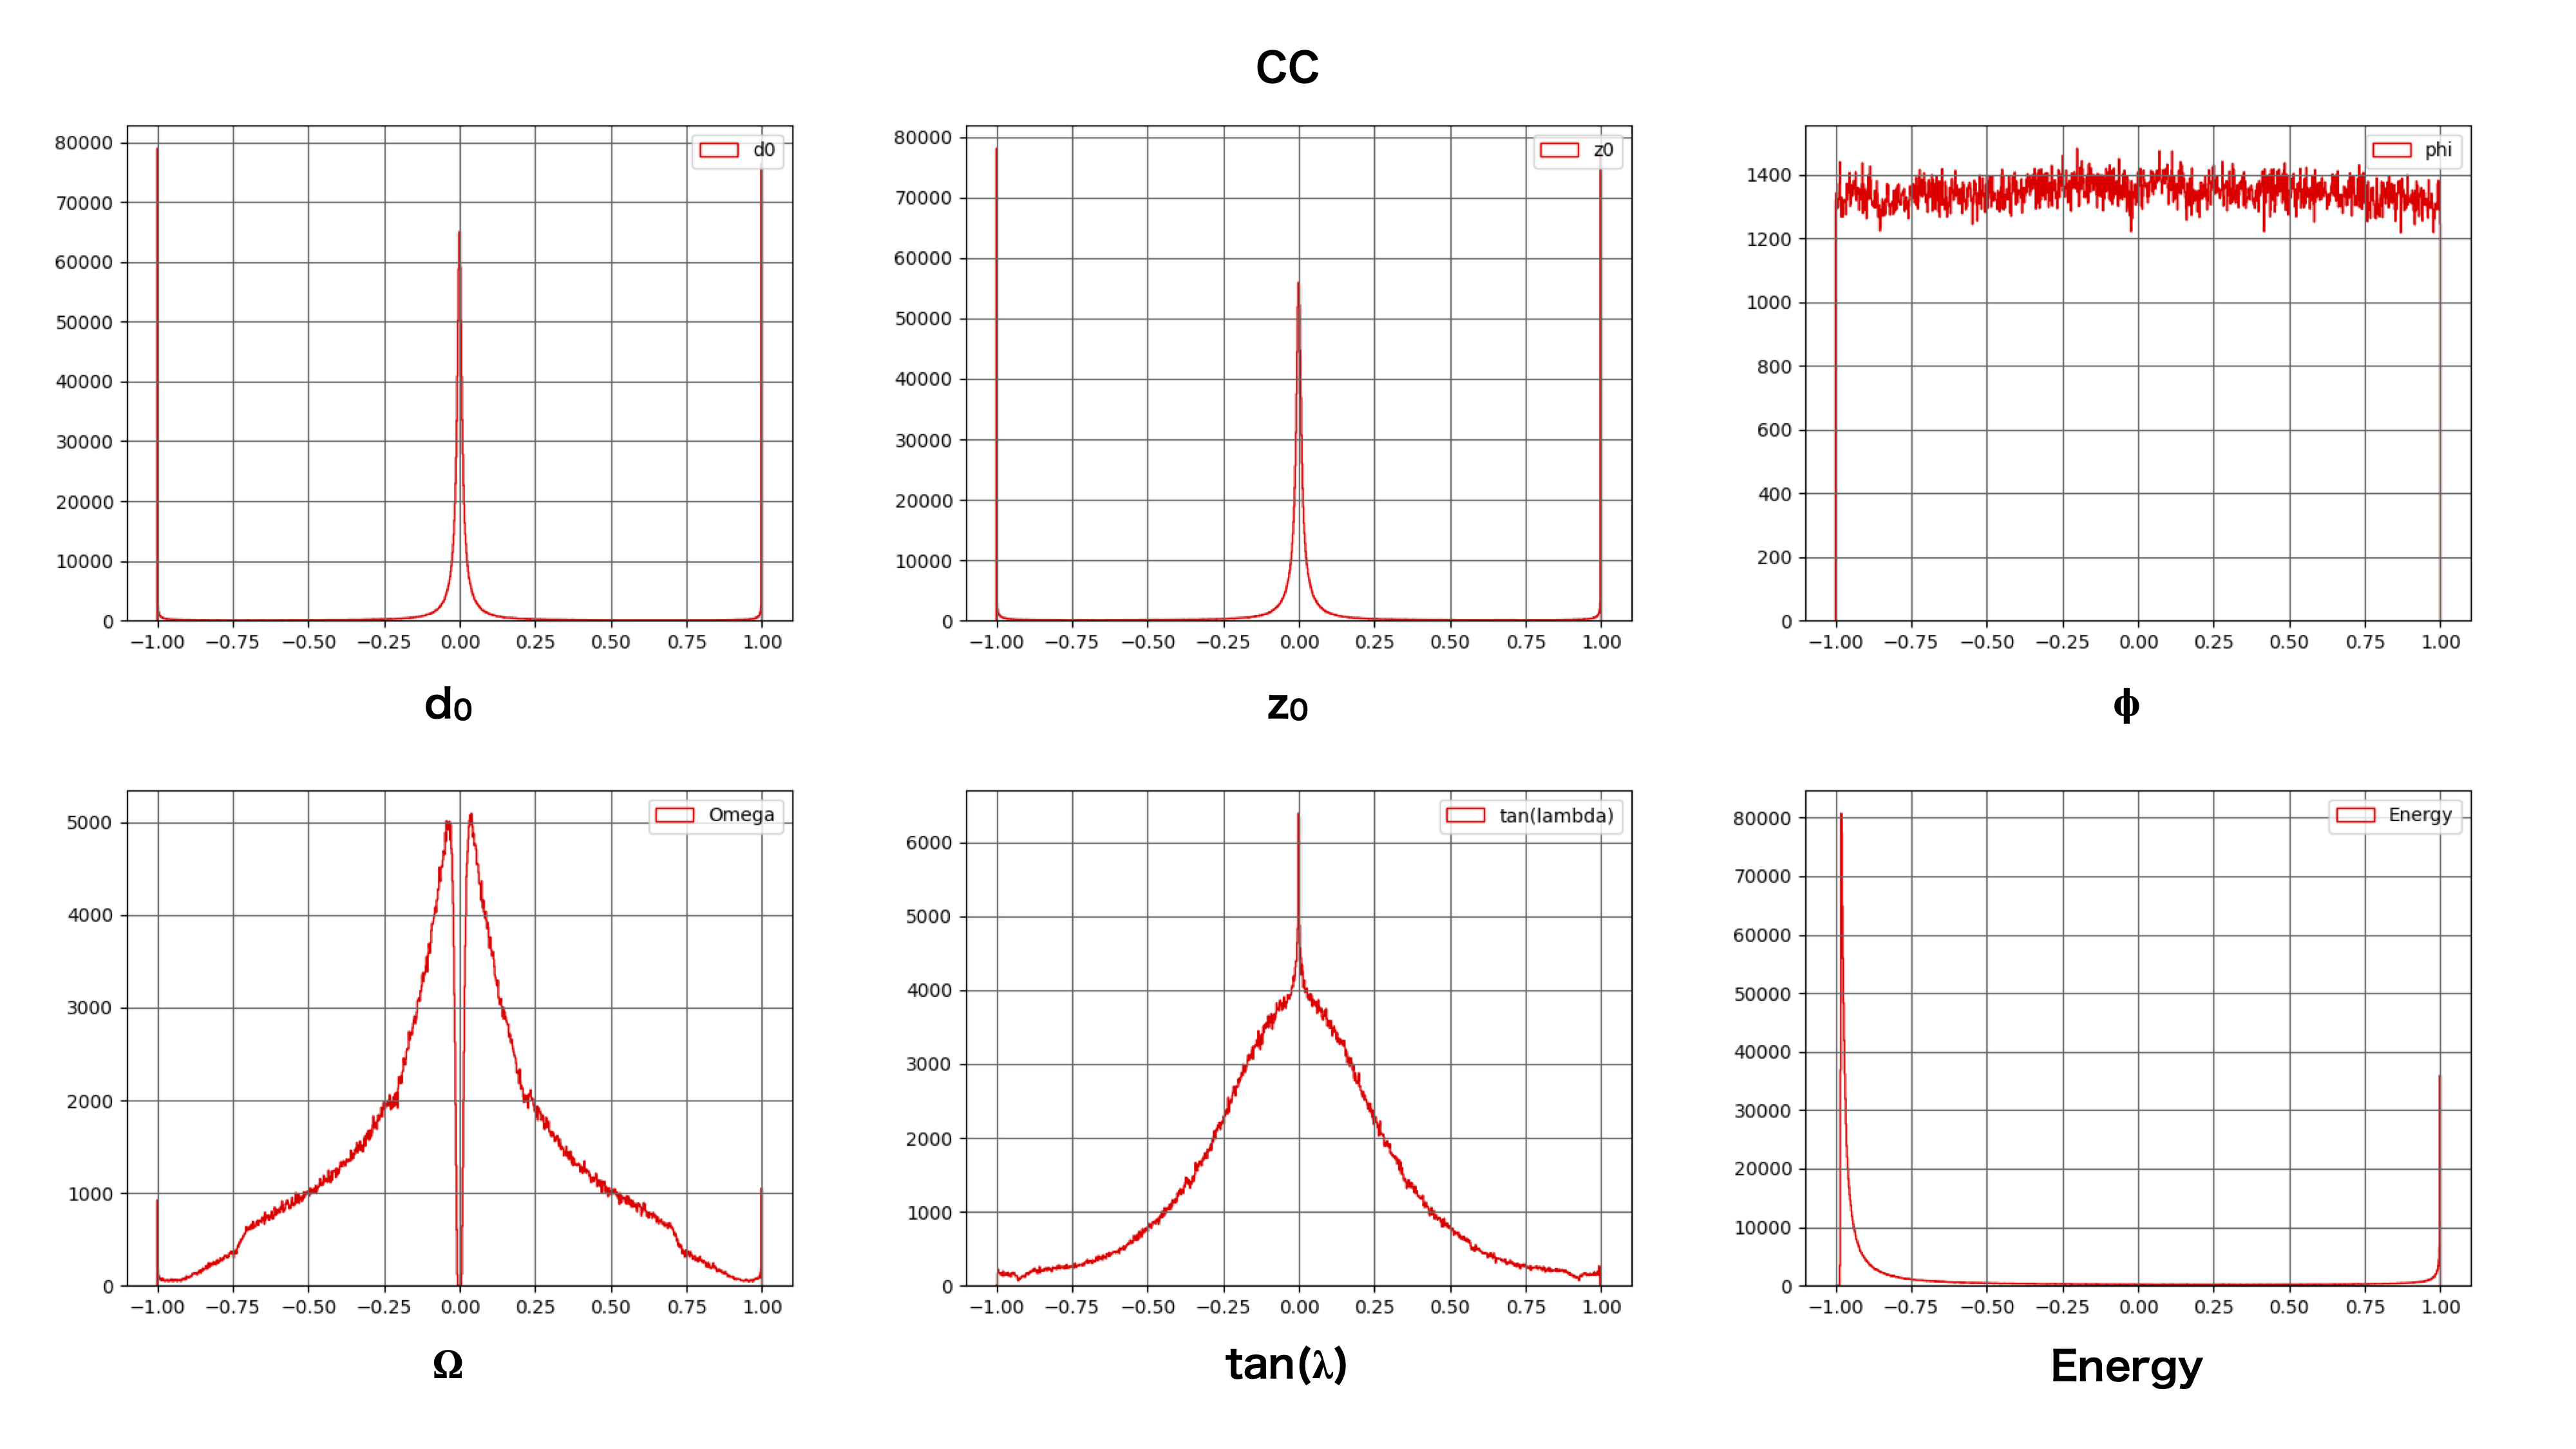
\includegraphics[width=1.0\textwidth, clip]{Figure/3Networks/3-1-2-1ReshapedVariablesCC.png}
    \subcaption{終状態$\rm c\bar{c}$での変換後の変数の分布}
    \label{3-1-2-1ReshapedVariablesCC}
   \end{minipage}
   \end{minipage}
  \caption{変数の分布の例}
  \label{3-1-2-1Variables}
 %\end{tabular}
\end{figure}

また、LCFIPlusのフィッティングで得られる変数であるカイ二乗や予想される崩壊点の位置についてもデータを用意した。
これらの値は1事象中の任意の二本の飛跡 (飛跡対) について計算を行ったものである。
ただし、深層学習の学習においてはこの値は基本的には使用せず、学習の健全性を確かめる目的や正解ラベルとして用いこととする。
MCの真値を用いて崩壊点の種類毎に分離したカイ二乗と予想される崩壊点の位置の分布を図\ref{}に示す。



(未完)

%%%%%%%%%%%%%%%%%%%%%%%%%%%%%%%%%%%%%%%%%%%%%%%%%%%%%%%%%%%%%%%%%%%%%%%%%%%%%%%%%%%%%%%%%%%%%%%%%%%%%
\section{深層学習を用いた崩壊点検出の実現} \label{Net:forVertexFinderwithDL}

\ref{chap:DeepLearning}章でも述べたように、深層学習は分類問題や回帰問題を解くことのできる教師あり学習である。
したがって、深層学習として問題を解く場合は、この二つのいずれかに問題を落とし込む必要がある。
我々はまずどのようにして、崩壊点検出を行うかを考えなければならない。
さて、\ref{Intro:SoftERILC:HighLevelEventReconstruction}章で述べた崩壊点検出の目的は、事象中の崩壊点とそこに属する飛跡を探索することである。
このような問題は一般に分類ではなく、クラスタリングのような手法によって解かれることが多い。
しかし、先述の\ref{Net:Data}節では、1事象に含まれる崩壊点の数と、飛跡の数が事象毎に異なっていることを示した。
そのような崩壊点の数や飛跡の数が不定であるというデータの性質を考慮した上で、崩壊点検出をクラスタリングで解くことはクラスター数や崩壊点種の差の扱いの面で不適であると判断した。
分類問題では、データの持つ特徴量の空間内である種の境界が引けなければならない。
そのため、あらゆるデータサンプルや事象内で不変な性質を考慮する必要がある。

以上を踏まえた上で私は二つのネットワークを用いた崩壊点検出を提案する。
一つは事象内のあらゆる飛跡対に対して、その飛跡対が結合 (Connected) しているか、非結合 (Not connected) であるか、結合しているならば、Primary VertexであるかSecondary Vertexであるかなどを分類するネットワークである。
これを「飛跡対についてのネットワーク」と呼ぶことにする。
飛跡対のついてのネットワークはあらゆる飛跡対に対して、崩壊点の種を探索することを目的としたネットワークである。
入力は飛跡二本分の情報であり、合計$44$個の変数である。
出力はデータサンプルの終状態によって分類数が変化してしまうが、基本的には崩壊点種 (非結合な飛跡対・Primary Vertex・Secondary Vertex) である。

飛跡対のついてのネットワークは崩壊点の種となる飛跡対を検出するだけであるので、単体では崩壊点を形成することはできない。
そこで、私は崩壊点の生成を行う、もう一つのネットワークを構築した。
これを「任意の数の飛跡についてのネットワーク」と呼ぶことにする。
任意の数の飛跡についてのネットワークは上記の飛跡対についてのネットワークによって得られた崩壊点の種に対して、事象中の飛跡を一本ずつ加え、それぞれの飛跡がその崩壊点の種と結合しているか、非結合であるかを分類するネットワークである。
そのようなネットワークを用いることで、最終的に事象中の全ての飛跡を考慮した崩壊点が生成される。
ただし、何度か述べているように事象中に含まれる飛跡の数は事象毎に異なるため、このようなネットワークは単純なフィードフォワードニューラルネットワークでは取り扱うことができない。
したがって私は、このネットワークをリカレントニューラルネットワークの技術を用いて作成した。

以上の二つのネットワークを用いるとこで、崩壊点検出を実現する。
構造や学習についてのより詳細な個々のネットワークの解説は、後の\ref{Net:PairModel}節や\ref{Net:VertexLSTM}節で述べる。

これらのネットワークはtensorflow/kerasフレームワークを用いて作成した。
また、学習に際しては弊研究室サーバーのTITAN RTXを二つと九州大学のスーパーコンピューターであるITOを使用した。
更に後述する推論の段階では更にC++への実装を行なっているが、その詳細に関しては\ref{Com:InferencewithCplusplus}節で述べる。

%%%%%%%%%%%%%%%%%%%%%%%%%%%%%%%%%%%%%%%%%%%%%%%%%%%%%%%%%%%%%%%%%%%%%%%%%%%%%%%%%%%%%%%%%%%%%%%%%%%%%
\section{飛跡対についてのネットワーク} \label{Net:PairModel}

ここでは\ref{Net:forVertexFinderwithDL}節で紹介した二つのネットワークの内、飛跡対についてのネットワークについて述べる。
主にネットワークの構造に関しては\ref{Net:PM:StructureofPM}項で、学習に関しては\ref{Net:PM:TrainingandStrategyofPM}項で解説する。
また、そのようにして構築、訓練されたネットワーク単体についての性能と評価に関しては、\ref{Net:PM:PerformanceofPM}項で述べることとする。

飛跡対についてのネットワークは、\ref{Net:forVertexFinderwithDL}述べたようにデータサンプルの終状態によって出力が異なる。
これは終状態が$\rm b\bar{b}$の場合はボトム ($\rm b$) ・フレーバーのSecondary Vertexとチャーム ($\rm c$) ・フレーバーのSecondary Vertexが生じるのに対し、終状態が$\rm c\bar{c}$の場合はチャーム ($\rm c$) ・フレーバーのSecondary Vertexのみが生じることに起因している。
また、終状態が$\rm b\bar{b}$の場合はボトムとチャーム・フレーバーのそれぞれのSecondary Vertex由来の飛跡対 (それぞれSecondary Vertex BB, Secondary Vertex CCと呼ぶこととする) と、更にボトム・フレーバーのSecondary Vertex由来の飛跡とそこから生じたチャーム・フレーバーのSecondary Vertex由来の飛跡を含んだ飛跡対 (Secondary Vertex BC) を考慮した。

\begin{figure}[h]
 \centering
 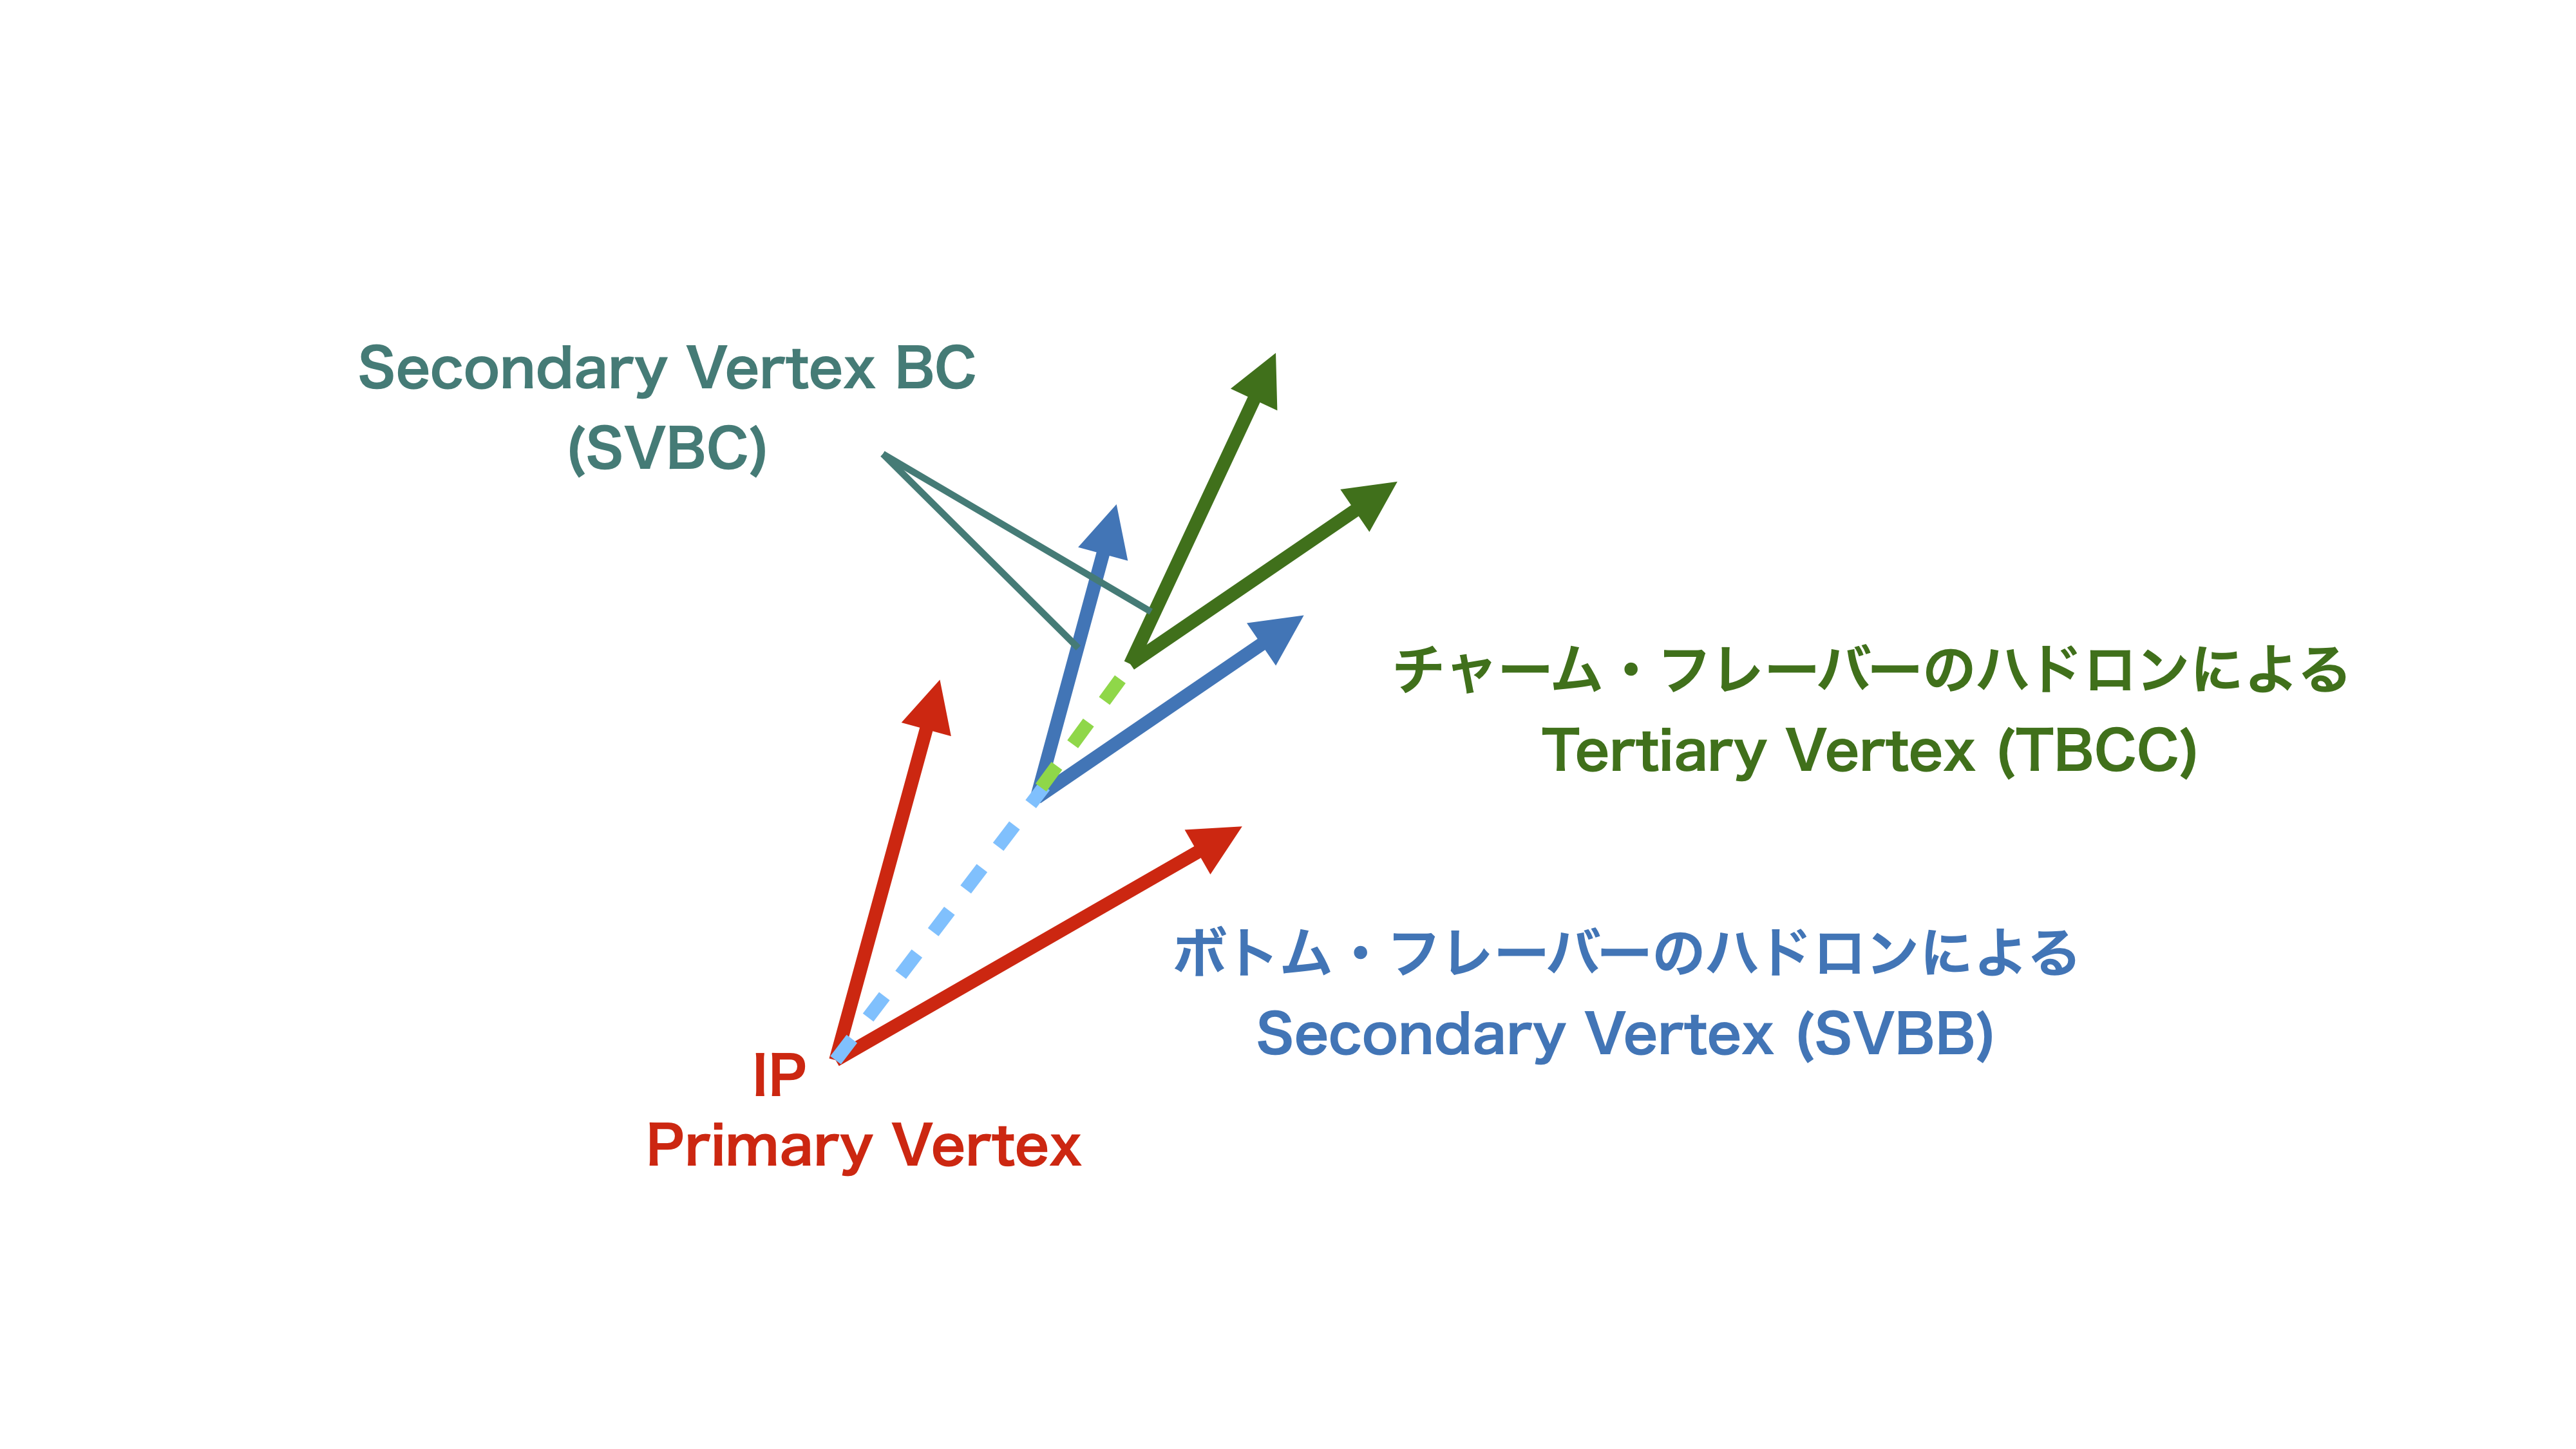
\includegraphics[trim = 0 100 0 50, width=0.9\textwidth]{Figure/3Networks/3-3-0-1SecondaryVertexBC.png}
 \caption{終状態$\rm b\bar{b}$での分類クラスの定義}
 \label{3-3-0-1SecondaryVertexBC}
\end{figure}

\begin{table}[htb]
 \centering
 \small
  \begin{tabular}{c c l} \hline
     終状態 & 分類クラス名\\ \hline \hline
    $\rm c\bar{c}$ & Not Connected, Primary Vertex, Secondary Vertex \\ \hline
    $\rm b\bar{b}$ & Not Connected, Primary Vertex, Secondary Vertex CC, BB, BC \\ \hline
  \end{tabular}
  \caption{終状態と分類クラス名}
  \label{FinalStateandClassName}
\end{table}

また、飛跡対について崩壊点の位置を予想するネットワークも全く同様の構造を用いて作成した。
こちらについては、訓練データの正解ラベルとしてLCFIPlusのフィッティングで得られる崩壊点の位置を用いた。
位置を予想するネットワークは\ref{Net:PM:PerformanceofPM}項での評価や\ref{chap:VertexFinderwithDL}章での崩壊点の種の選別に使用している。


%%%%%%%%%%%%%%%%%%%%%%%%%%%%%%%%%%%%%%%%%%%%%%%%%%%%%%%%%%%%%%%%%%%%%%%%
\subsection{ネットワークの構造} \label{Net:PM:StructureofPM}

飛跡対についてのネットワークは非常にシンプルなフィードフォーワードニューラルネットワーク構造のものを使用した。
ネットワークの概略図を図\ref{3-3-1-1PairModel}に示す。

\begin{figure}[h]
 \centering
 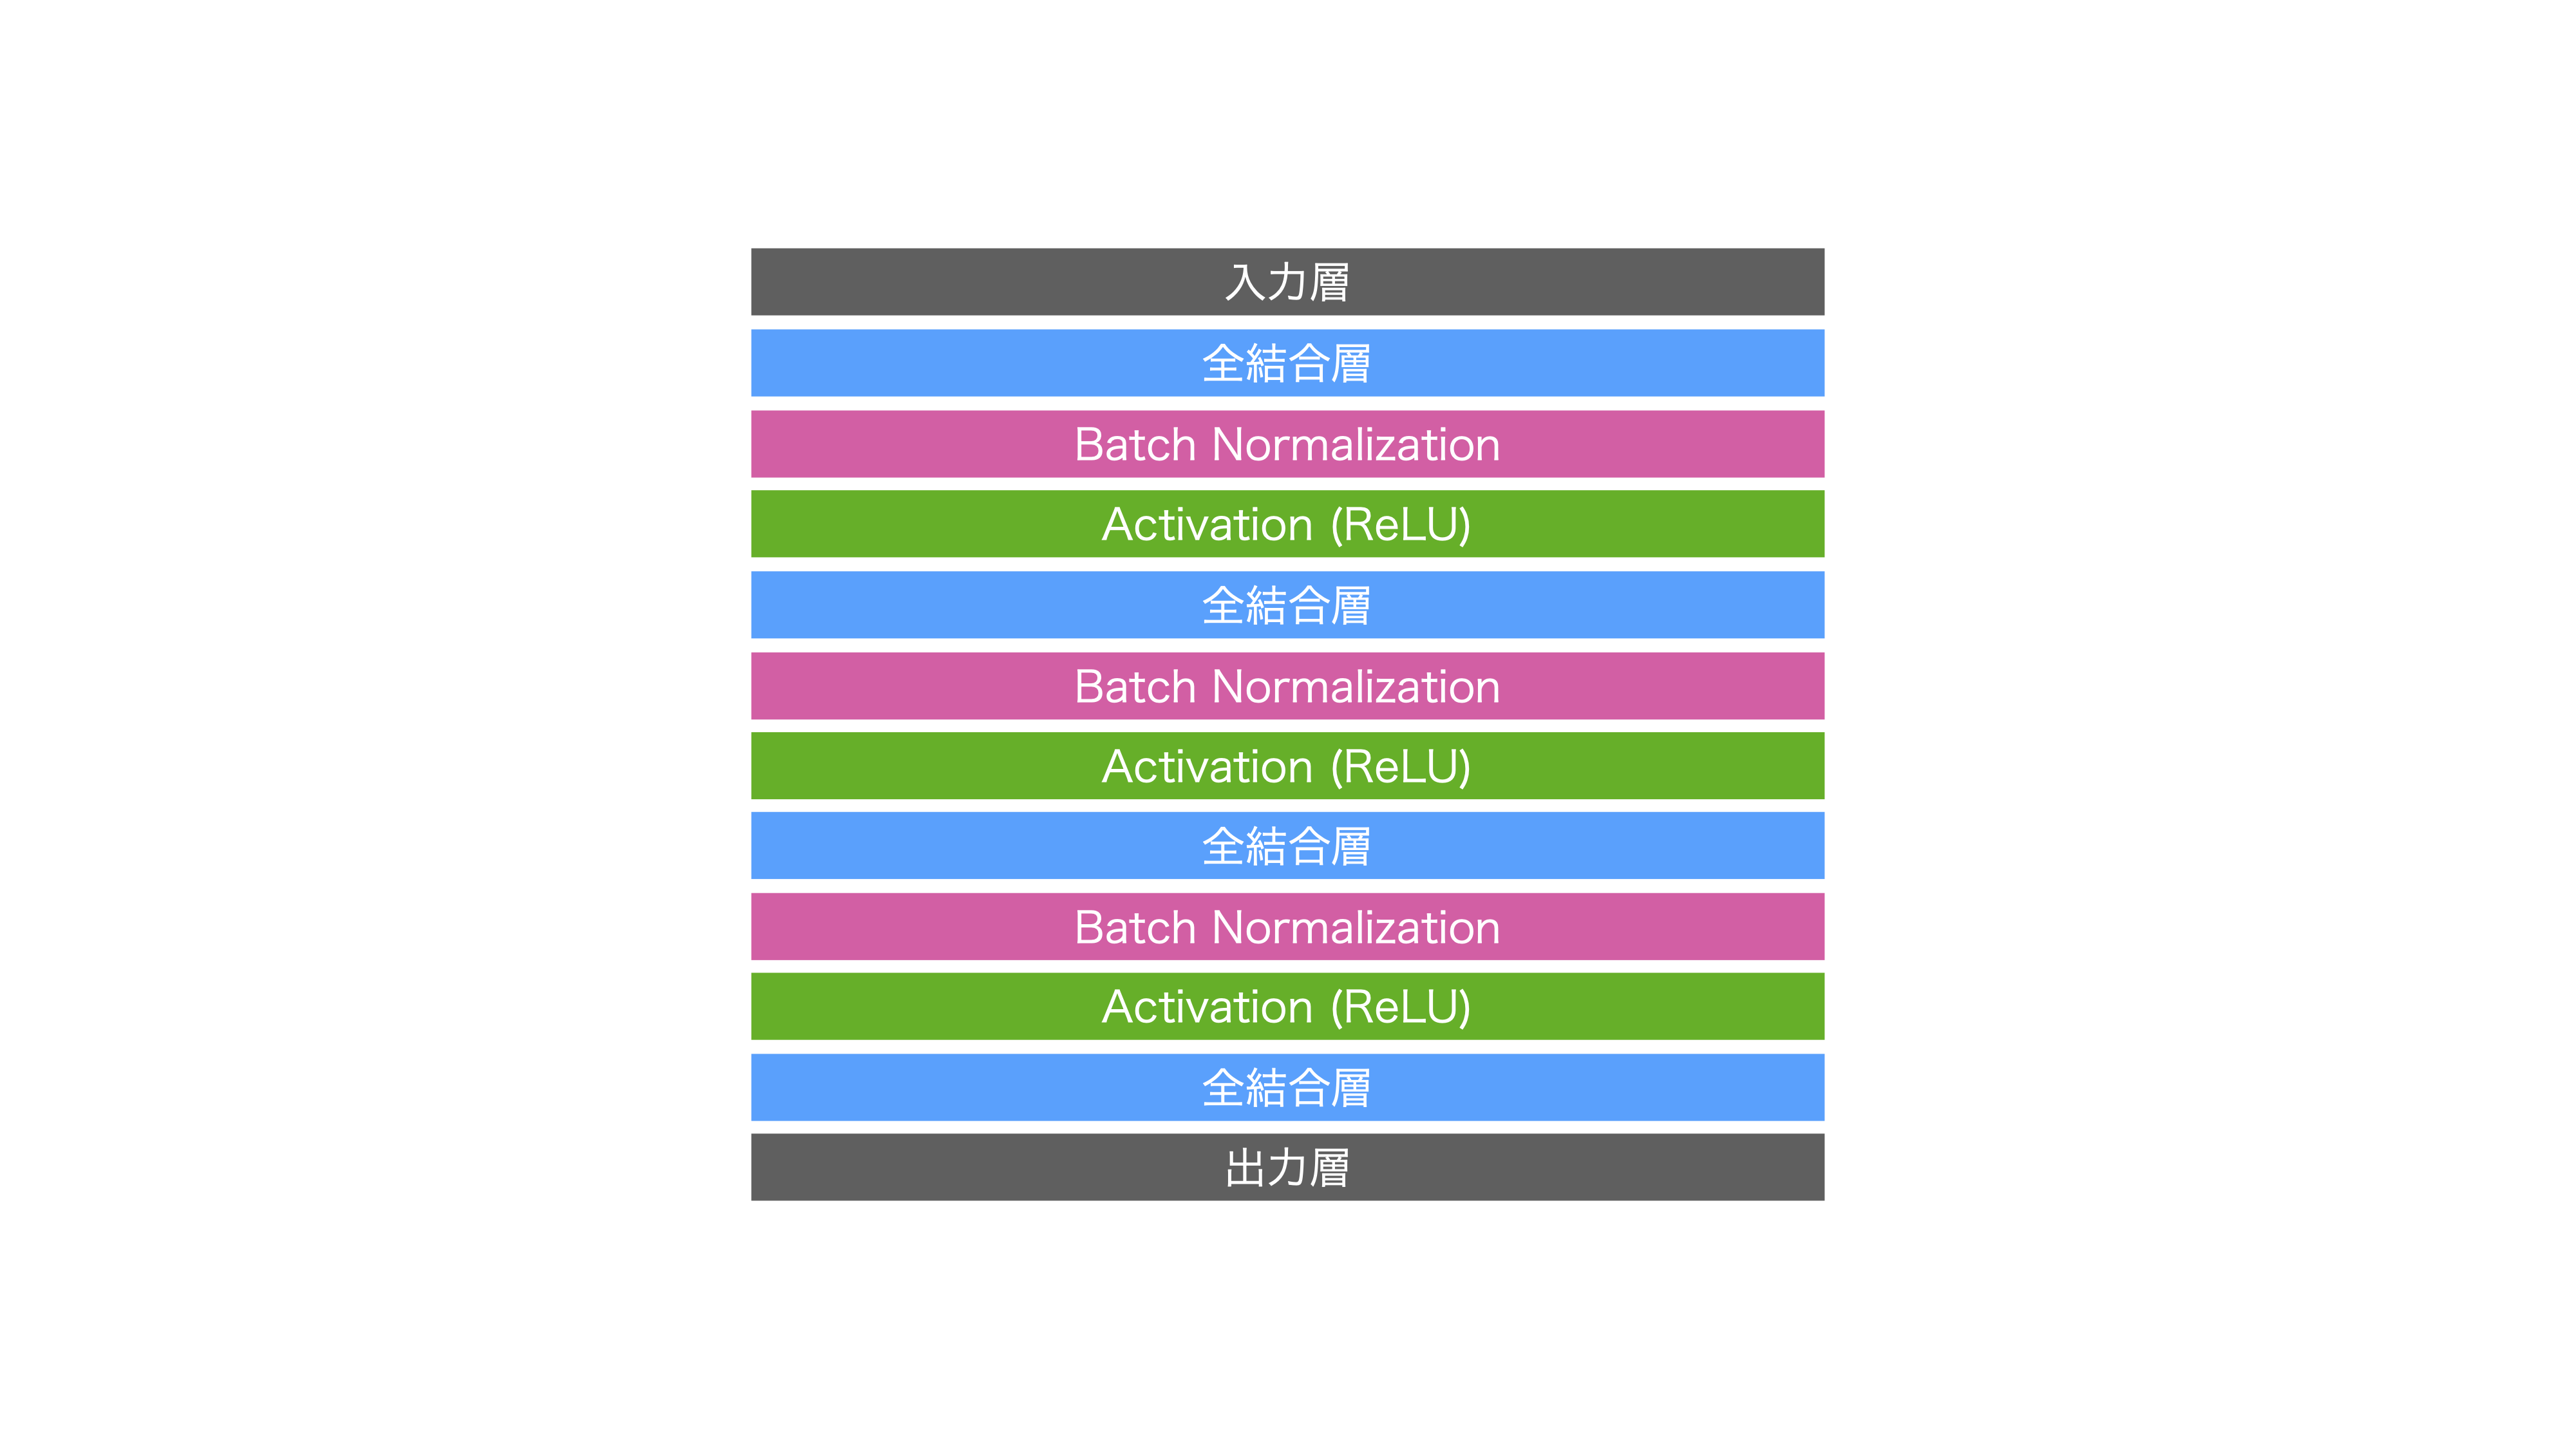
\includegraphics[trim = 100 100 100 50, width=0.9\textwidth]{Figure/3Networks/3-3-1-1PairModel.png}
 \caption{飛跡対についてのネットワークの概略図}
 \label{3-3-1-1PairModel}
\end{figure}

終状態や崩壊点種、位置を予想する際のネットワークの違いは最後の全結合層のノード数をそれぞれ終状態$\rm b\bar{b}$では$5$、$\rm c\bar{c}$では$3$、位置を予想する場合は回帰問題として解くためノード数を$1$とした。
標準的なハイパーパラメータは図\ref{3-3-1-2PairModelSummary}にまとめている。

\begin{figure}[h]
 \centering
 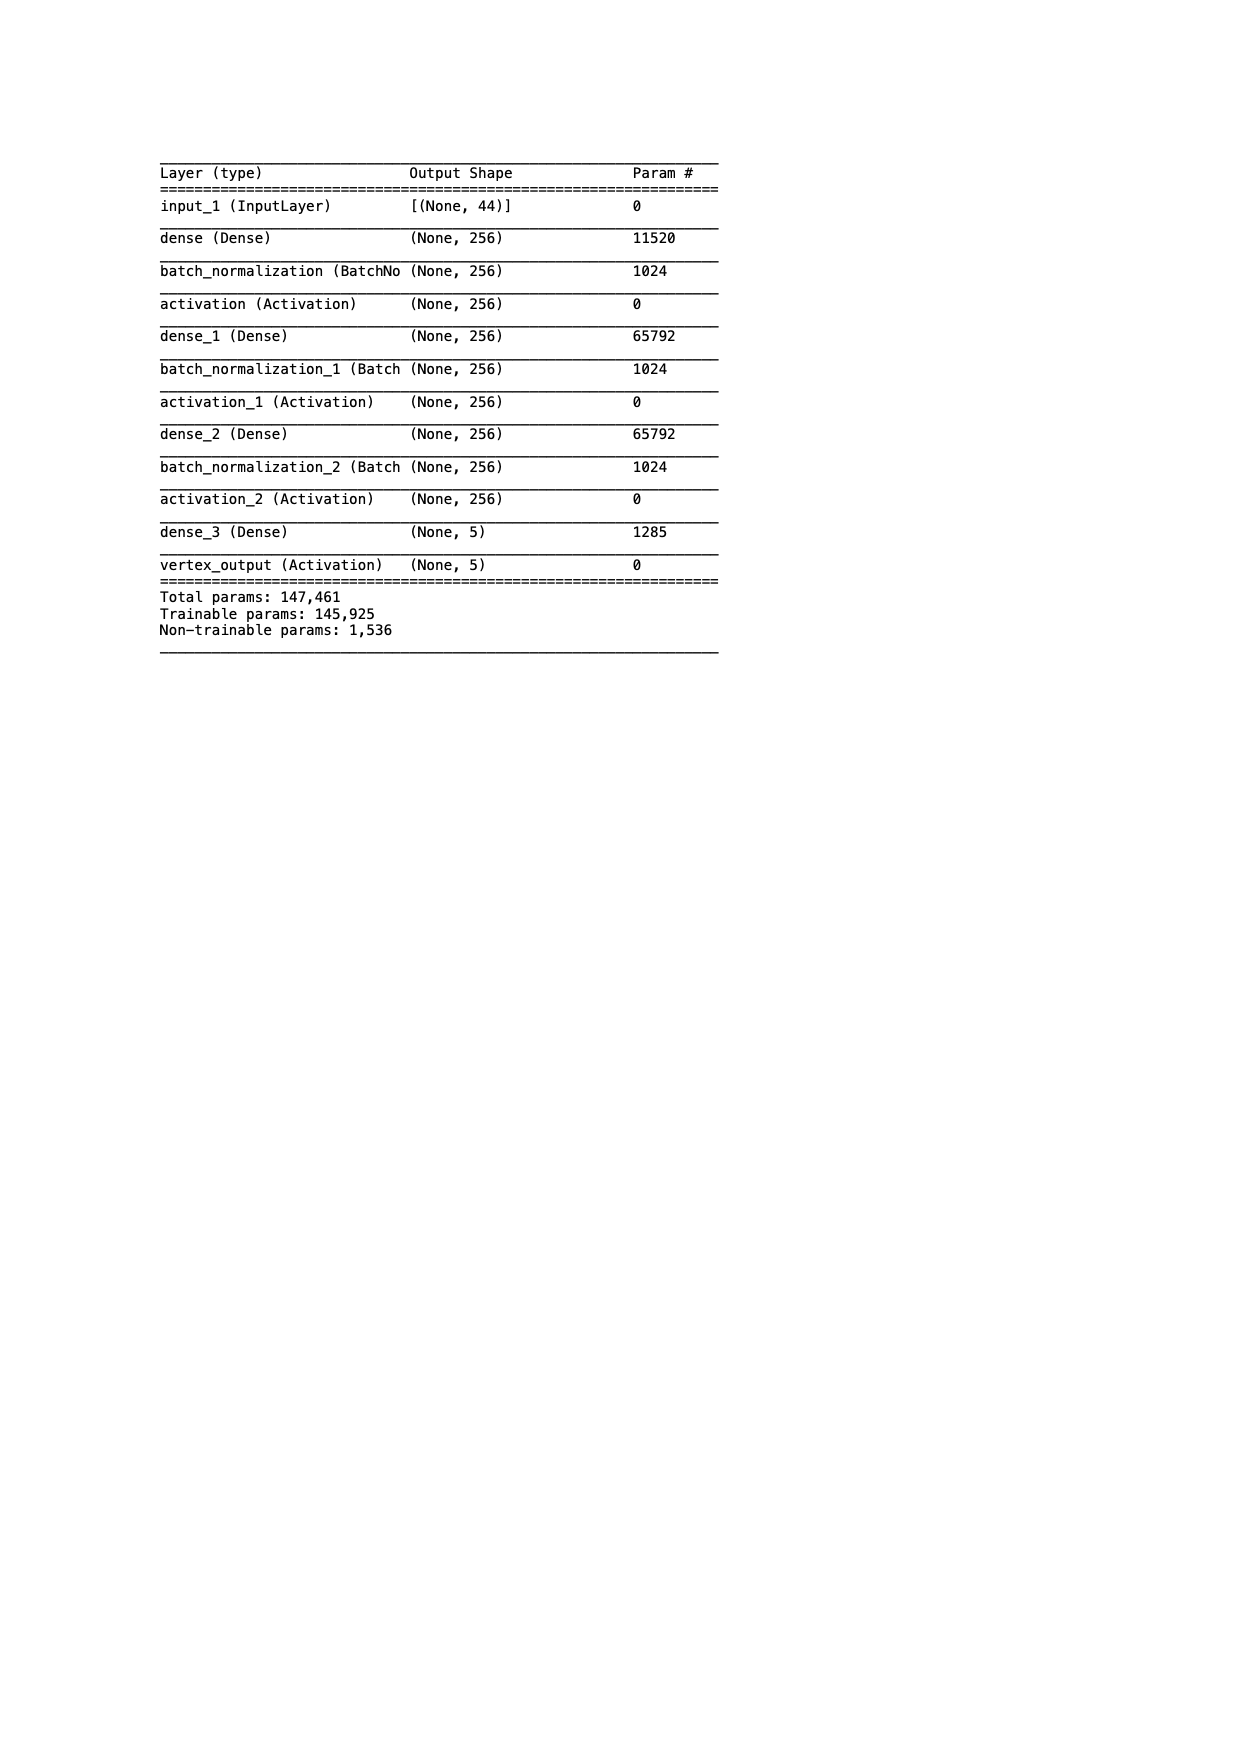
\includegraphics[trim = 75 500 125 0, width=0.9\textwidth]{Figure/3Networks/3-3-1-2PairModelSummary.png}
 \caption{$b\bar{b}$データセットについて崩壊点種予測モデルにおける各種パラメーターの出力}
 \label{3-3-1-2PairModelSummary}
\end{figure}

また、過学習 (Over fitting) を避ける為、Batch Normalization\cite{BatchNormalizationpaper}を全結合層の後ろに配置している。
過学習とは、ネットワークが過度に訓練データに適合してしまい、検証データやテストデータへの汎化性能が悪化してしまう教師あり学習での問題である。
また勾配消失への対策として、活性化関数は全てReLU関数を使用している。
ノード数や層数に関してのハイパーパラメータ・チューニングに関しては\ref{Net:PM:PerformanceofPM}にて述べる。


%%%%%%%%%%%%%%%%%%%%%%%%%%%%%%%%%%%%%%%%%%%%%%%%%%%%%%%%%%%%%%%%%%%%%%%%
\subsection{ネットワークの学習と戦略} \label{Net:PM:TrainingandStrategyofPM}

訓練データは事象中の全ての飛跡対の組み合わせを考える。
したがって図\ref{}のように、分類クラスの数の比は"Not Connected"が支配的な不均衡 (Imbalanced) データとなる。
このような不均衡データについては、少数クラスのデータをかさ増しするOversampling、多数クラスのデータを間引くUndersampling、損失関数のコストに重みをつけるコスト考慮型学習の主に三つの対応策が存在する。

OversamplingやUndersamplingは過学習や情報の欠損などの問題を孕んでいるため、本研究ではコスト考慮型学習を用いた。
また重みは分類クラスの数の比の逆数を使用した。

\begin{itemize}
 \item 終状態$\rm b\bar{b}$\\
\begin{equation}
 \begin{split}
 L = &- t_{\rm NC} \log{(y_{\rm NC})} -  t_{\rm PV} \log{(y_{\rm PV})} -  t_{\rm SVCC} \log{(y_{\rm SVCC})}\\
       &-  t_{\rm SVBB} \log{(y_{\rm SVBB})} -  t_{\rm SVBC} \log{(y_{\rm SVBC})}\\
 \end{split}
\end{equation}
 \item 終状態$\rm c\bar{c}$\\
\begin{equation}
 L = - t_{\rm NC} \log{(y_{\rm NC})} -  t_{\rm PV} \log{(y_{\rm PV})} -  t_{\rm SV} \log{(y_{\rm SV})}
\end{equation}
\end{itemize}
ここで、${\rm NC:\ Not\ Connected,\ PV:\ Primary\ Vertex,\ SV:\ Secondary Vertex}$と訳した。

次に重み更新の最適化手法として、SGDを用いた。
これは、Adamなどでは収束が早すぎ、過学習になる恐れがあったためである。

エポックを横軸に、正答率と損失を縦軸にプロットしたものを図\ref{}に示す。


%%%%%%%%%%%%%%%%%%%%%%%%%%%%%%%%%%%%%%%%%%%%%%%%%%%%%%%%%%%%%%%%%%%%%%%%
\subsection{ネットワークの性能} \label{Net:PM:PerformanceofPM}

飛跡対についてのネットワークの性能を混合行列 (Confusion Matrix) にまとめる。(図\ref{})

位置を見ているか\\
Chi2, Pos, Cov Mat, 位置を予想するネットワーク\\

Othersクラスを加えた分類\\

ROCカーブ\\


%%%%%%%%%%%%%%%%%%%%%%%%%%%%%%%%%%%%%%%%%%%%%%%%%%%%%%%%%%%%%%%%%%%%%%%%%%%%%%%%%%%%%%%%%%%%%%%%%%%%%
\section{任意の数の飛跡についてのネットワーク} \label{Net:VertexLSTM}

ここでは\ref{Net:forVertexFinderwithDL}節で紹介した二つのネットワークの内、任意の数の飛跡のためのネットワークについて述べる。
基本的には前節の飛跡対についてのネットワークと同様の手順での解説を行うが、この任意の数の飛跡についてのネットワークは、既存のネットワーク構造にはない独自のネットワークで構築している。
これは本研究におけるデータの特殊性や問題解決のための最適なネットワークを考慮した結果である。
このようなネットワークの詳細な構造については\ref{Net:VLSTM:DetailedStructureofVLSTM}項で述べる。


%%%%%%%%%%%%%%%%%%%%%%%%%%%%%%%%%%%%%%%%%%%%%%%%%%%%%%%%%%%%%%%%%%%%%%%%
\subsection{ネットワークの構造} \label{Net:VLSTM:StructureofVLSTM}

任意の数の飛跡についてのネットワークではリカレントニューラルネットワークの技術を採用している。
ただし、飛跡は本質的に順序を持っておらず、系列データではない為、リカレントニューラルネットワークをそのまま用いることはデータの性質に合わない。
この為私は、リカレントニューラルネットワークの一つであるLSTMを拡張し、新しい独自のリカレントニューラルネットワークの構造を構築した。
この独自のネットワーク構造については、次項\ref{Net:VLSTM:DetailedStructureofVLSTM}にて解説する。
ここでは、より大きな枠組みとしてのネットワークの構造について述べる。

図\ref{3-4-1-1SimpleVLSTM}は、リカレントニューラルネットワークを用いた最も簡単な崩壊点生成を表現したものである。
ここで、左から崩壊点の種である飛跡対が入力されている。
実際には全結合層を通し、リカレントニューラルネットワークの初期状態としている。
この初期状態は、リカレントニューラルネットワーク内の重みと共に全結合層が学習される為、学習可能な初期状態 (Trainable (Learnable) Initial State) となっている。
また、飛跡は下から一本ずつ入力され、1事象分の全ての飛跡が使用されるが、リカレントニューラルネットワークである為、系列として扱う飛跡の本数は任意である。
したがって、ある崩壊点のタネに対して、任意の数の飛跡が結合しているか否かを分類することができる。

\begin{figure}[h]
 \centering
 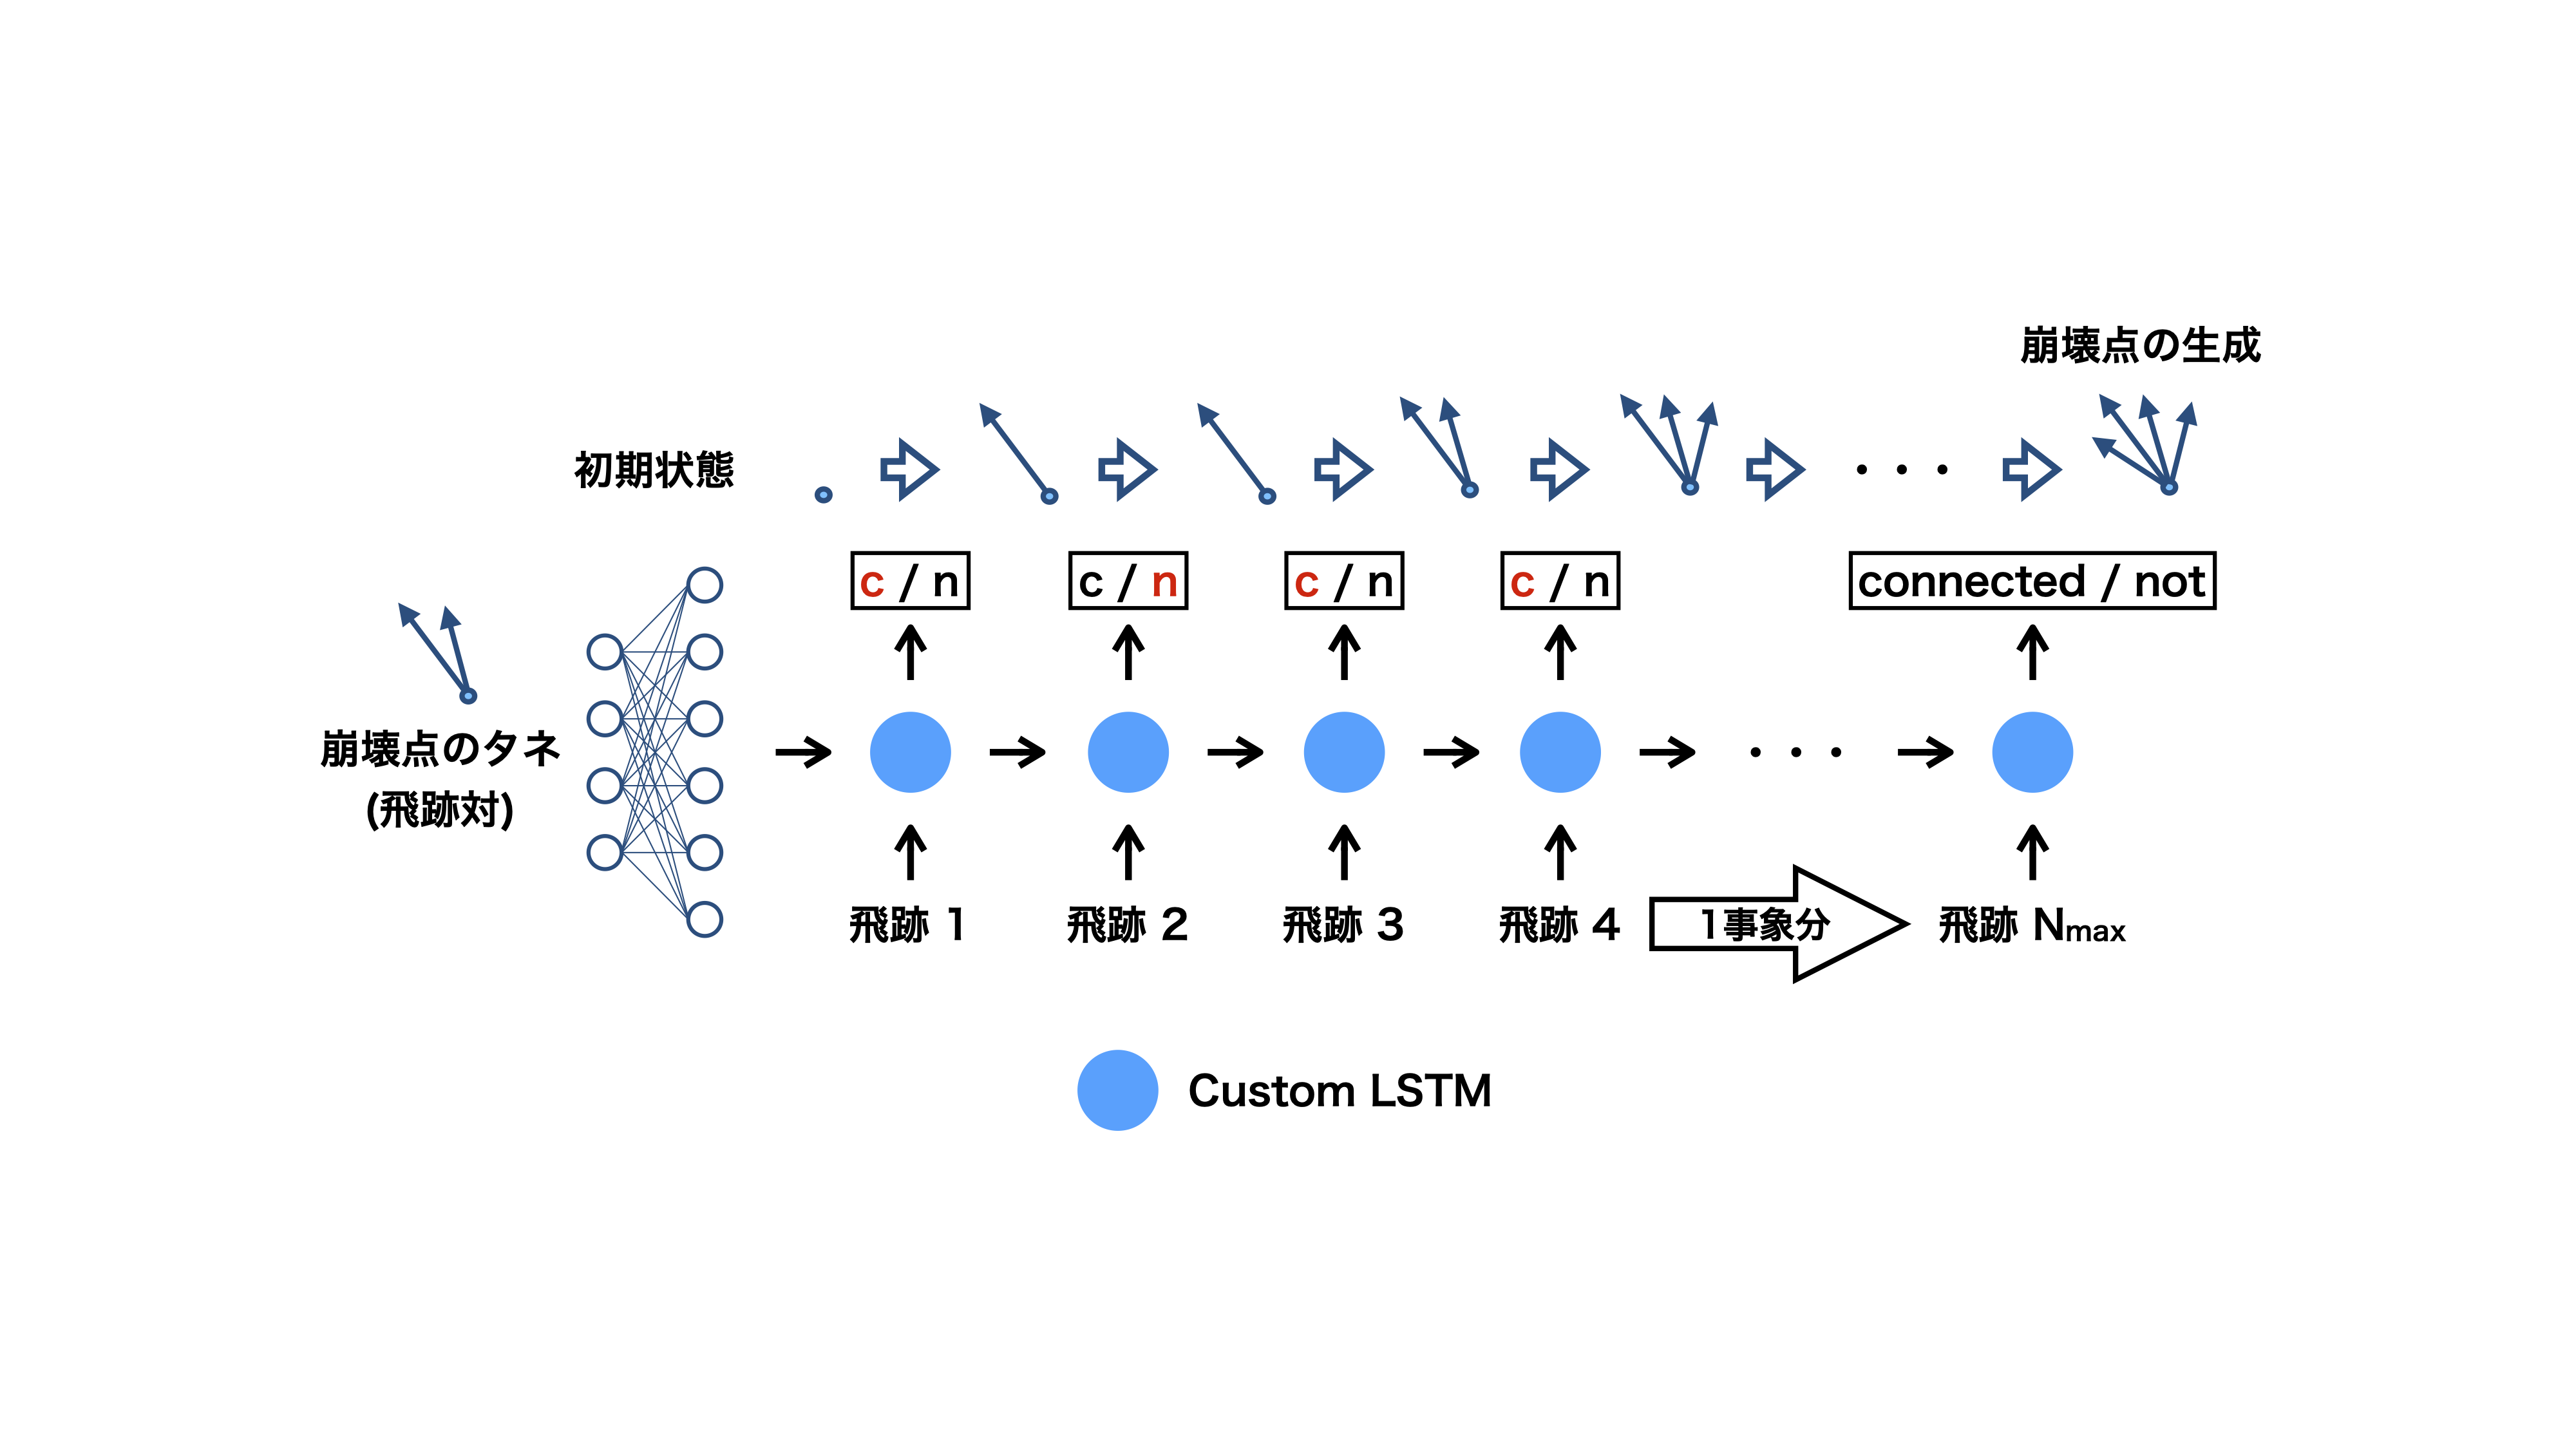
\includegraphics[trim = 0 80 0 0, width=1.0\textwidth]{Figure/3Networks/3-4-1-1SimpleVLSTM.png}
 \caption{独自のリカレントニューラルネットワーク構造を用いた崩壊点の生成}
 \label{3-4-1-1SimpleVLSTM}
\end{figure}

自然な発想として、今、飛跡について1事象分 (系列) の全ての情報を持っている為、エンコーダー・デコーダーモデルとすることで、その事象についての情報 (コンテキスト) を活用することができる。
更に、エンコーダー・デコーダーモデルの間にAttentionを組み込むことも同様に自然な発想である。
その様なネットワークを図\ref{3-4-1-2EncoderDecoderVLSTM}に示す。
この図では上から飛跡が入力されており、崩壊点の種である飛跡対は上部左右と左下から入力されている。
上部がエンコーダー部、下部がデコーダ部である。
個々の基本的な構造は図\ref{3-4-1-1SimpleVLSTM}と同一であるが、エンコーダー部には双方向リカレントニューラルネットワークを採用している。
また、デコーダー部では独自のリカレントニューラルネットワークの構造を更に拡張し、エンコーダー部の出力を初期状態の一つとしてAttentionに対応させたネットワークを使用している。
詳細は次項\ref{Net:VLSTM:DetailedStructureofVLSTM}にて述べる。

Attentionを組み込むことによって、デコーダー部の"ある"飛跡はエンコーダー部によって抽出された飛跡の情報に任意の注意を払って、1事象分の情報を取得することになる。
エンコーダー・デコーダーモデルに拡張しても、このネットワークの基本構造がリカレントニューラルネットワークであることに変わりがない為、デコーダー部の飛跡の本数を任意に変えることが可能である。

\begin{figure}[h]
 \centering
 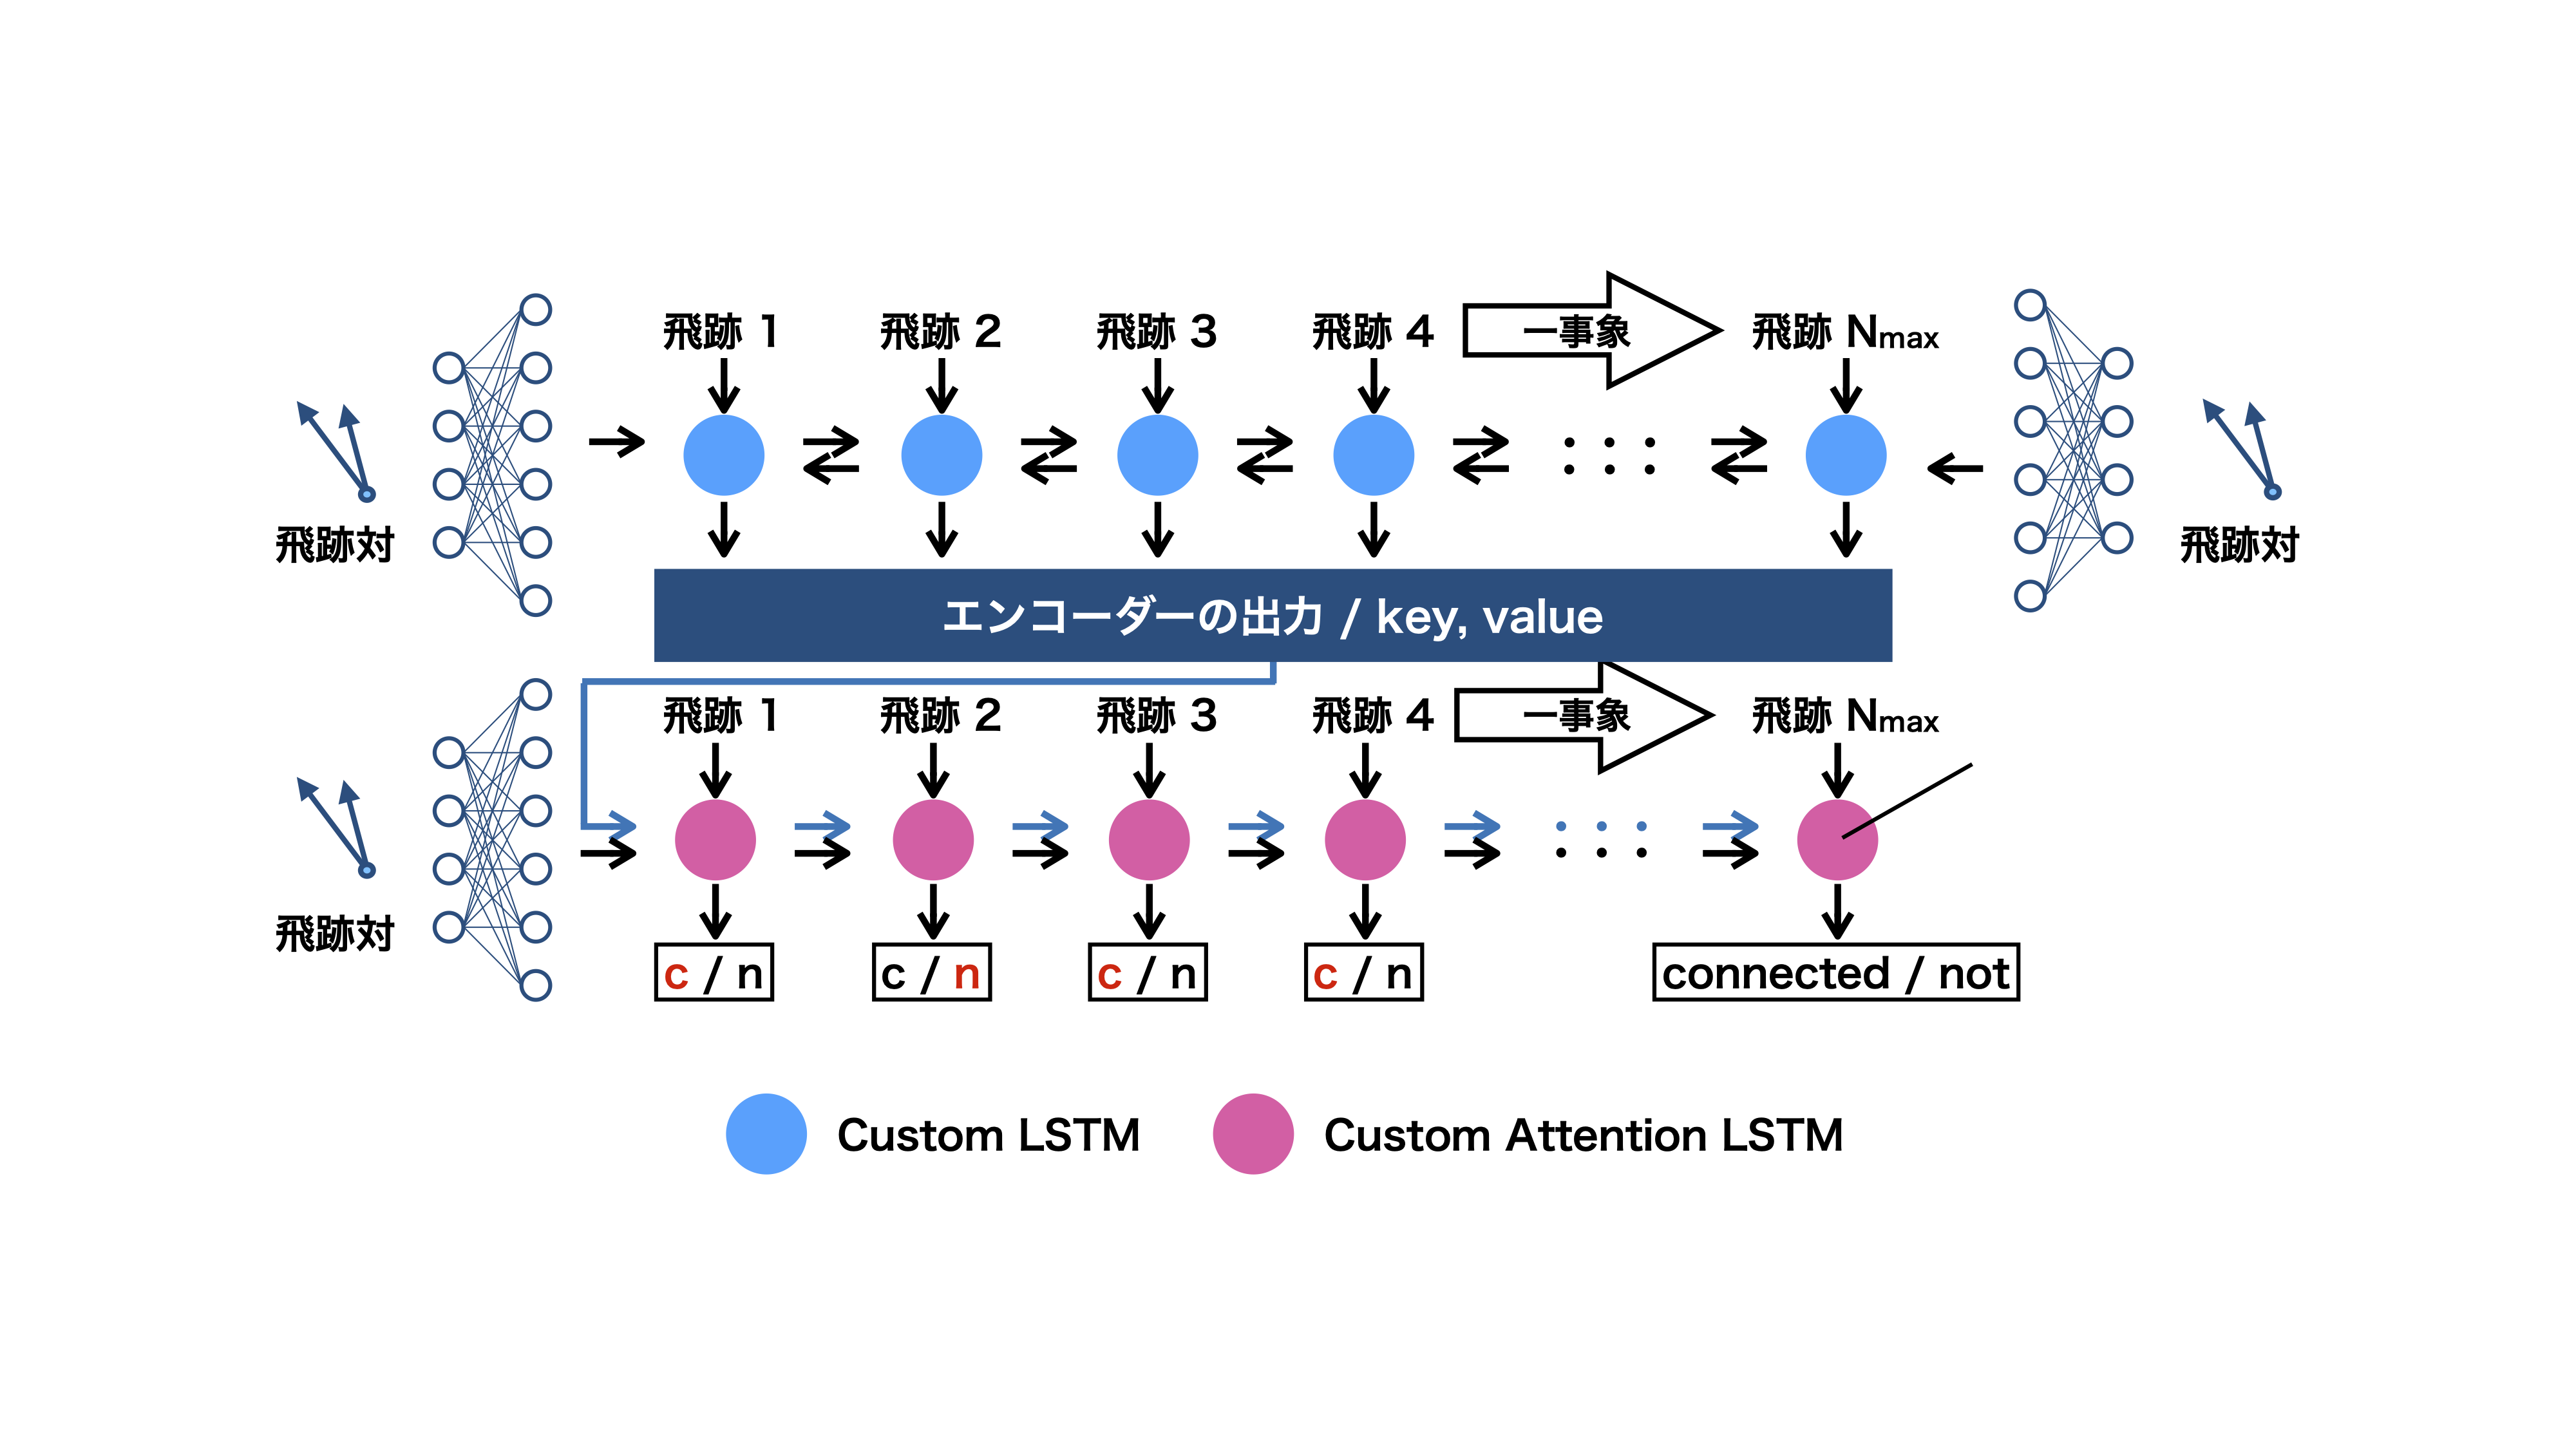
\includegraphics[trim = 0 80 0 0, width=1.0\textwidth]{Figure/3Networks/3-4-1-2EncoderDecoderVLSTM.png}
 \caption{Attentionを用いたエンコーダー・デコーダーモデルへの拡張}
 \label{3-4-1-2EncoderDecoderVLSTM}
\end{figure}

\begin{figure}[h]
 \centering
 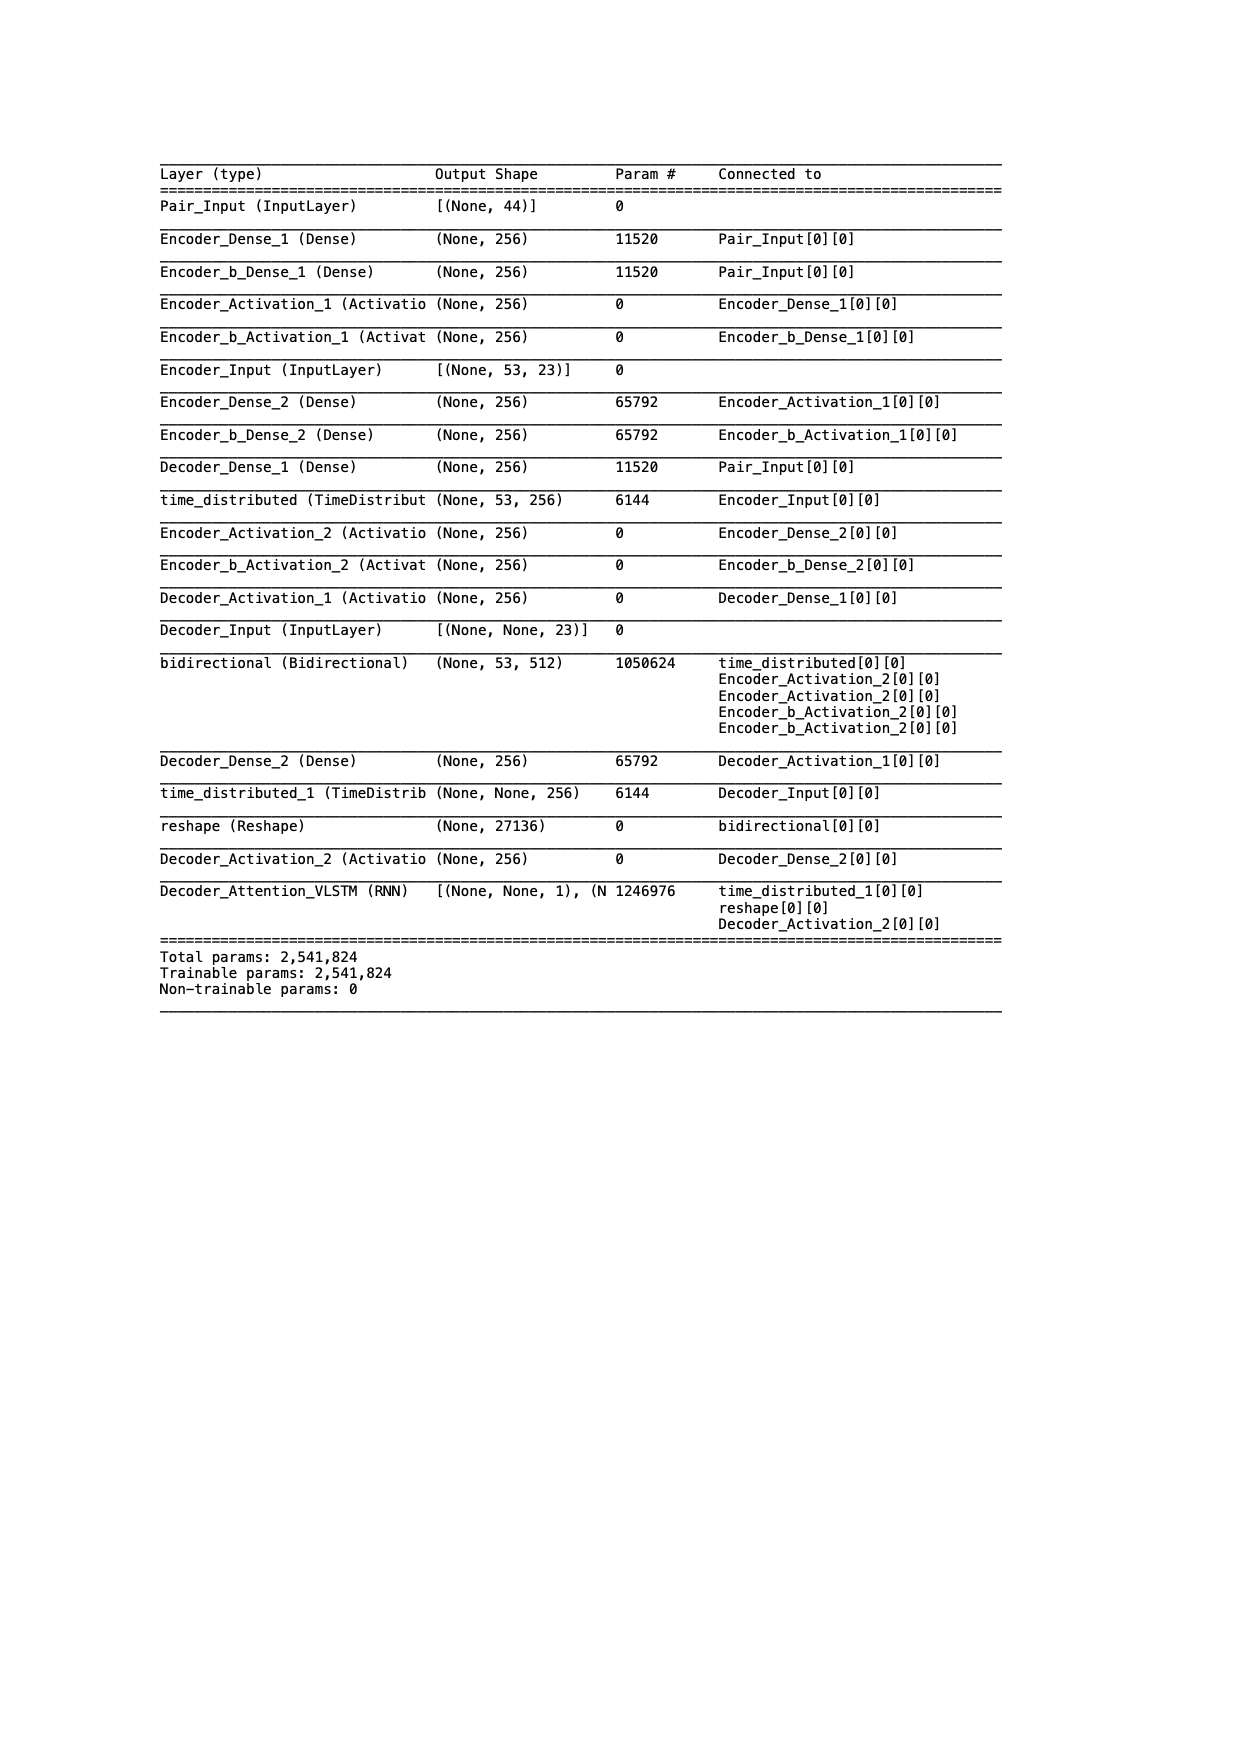
\includegraphics[trim = 75 300 125 0, width=0.9\textwidth]{Figure/3Networks/3-4-1-3VLSTMSummary.png}
 \caption{エンコーダー・デコーダーモデルにおける各種パラメーターの出力}
 \label{3-4-1-3VLSTMSummary}
\end{figure}


%%%%%%%%%%%%%%%%%%%%%%%%%%%%%%%%%%%%%%%%%%%%%%%%%%%%%%%%%%%%%%%%%%%%%%%%
\subsection{ネットワークの詳細な構造} \label{Net:VLSTM:DetailedStructureofVLSTM}

\begin{figure}[h]
 \centering
 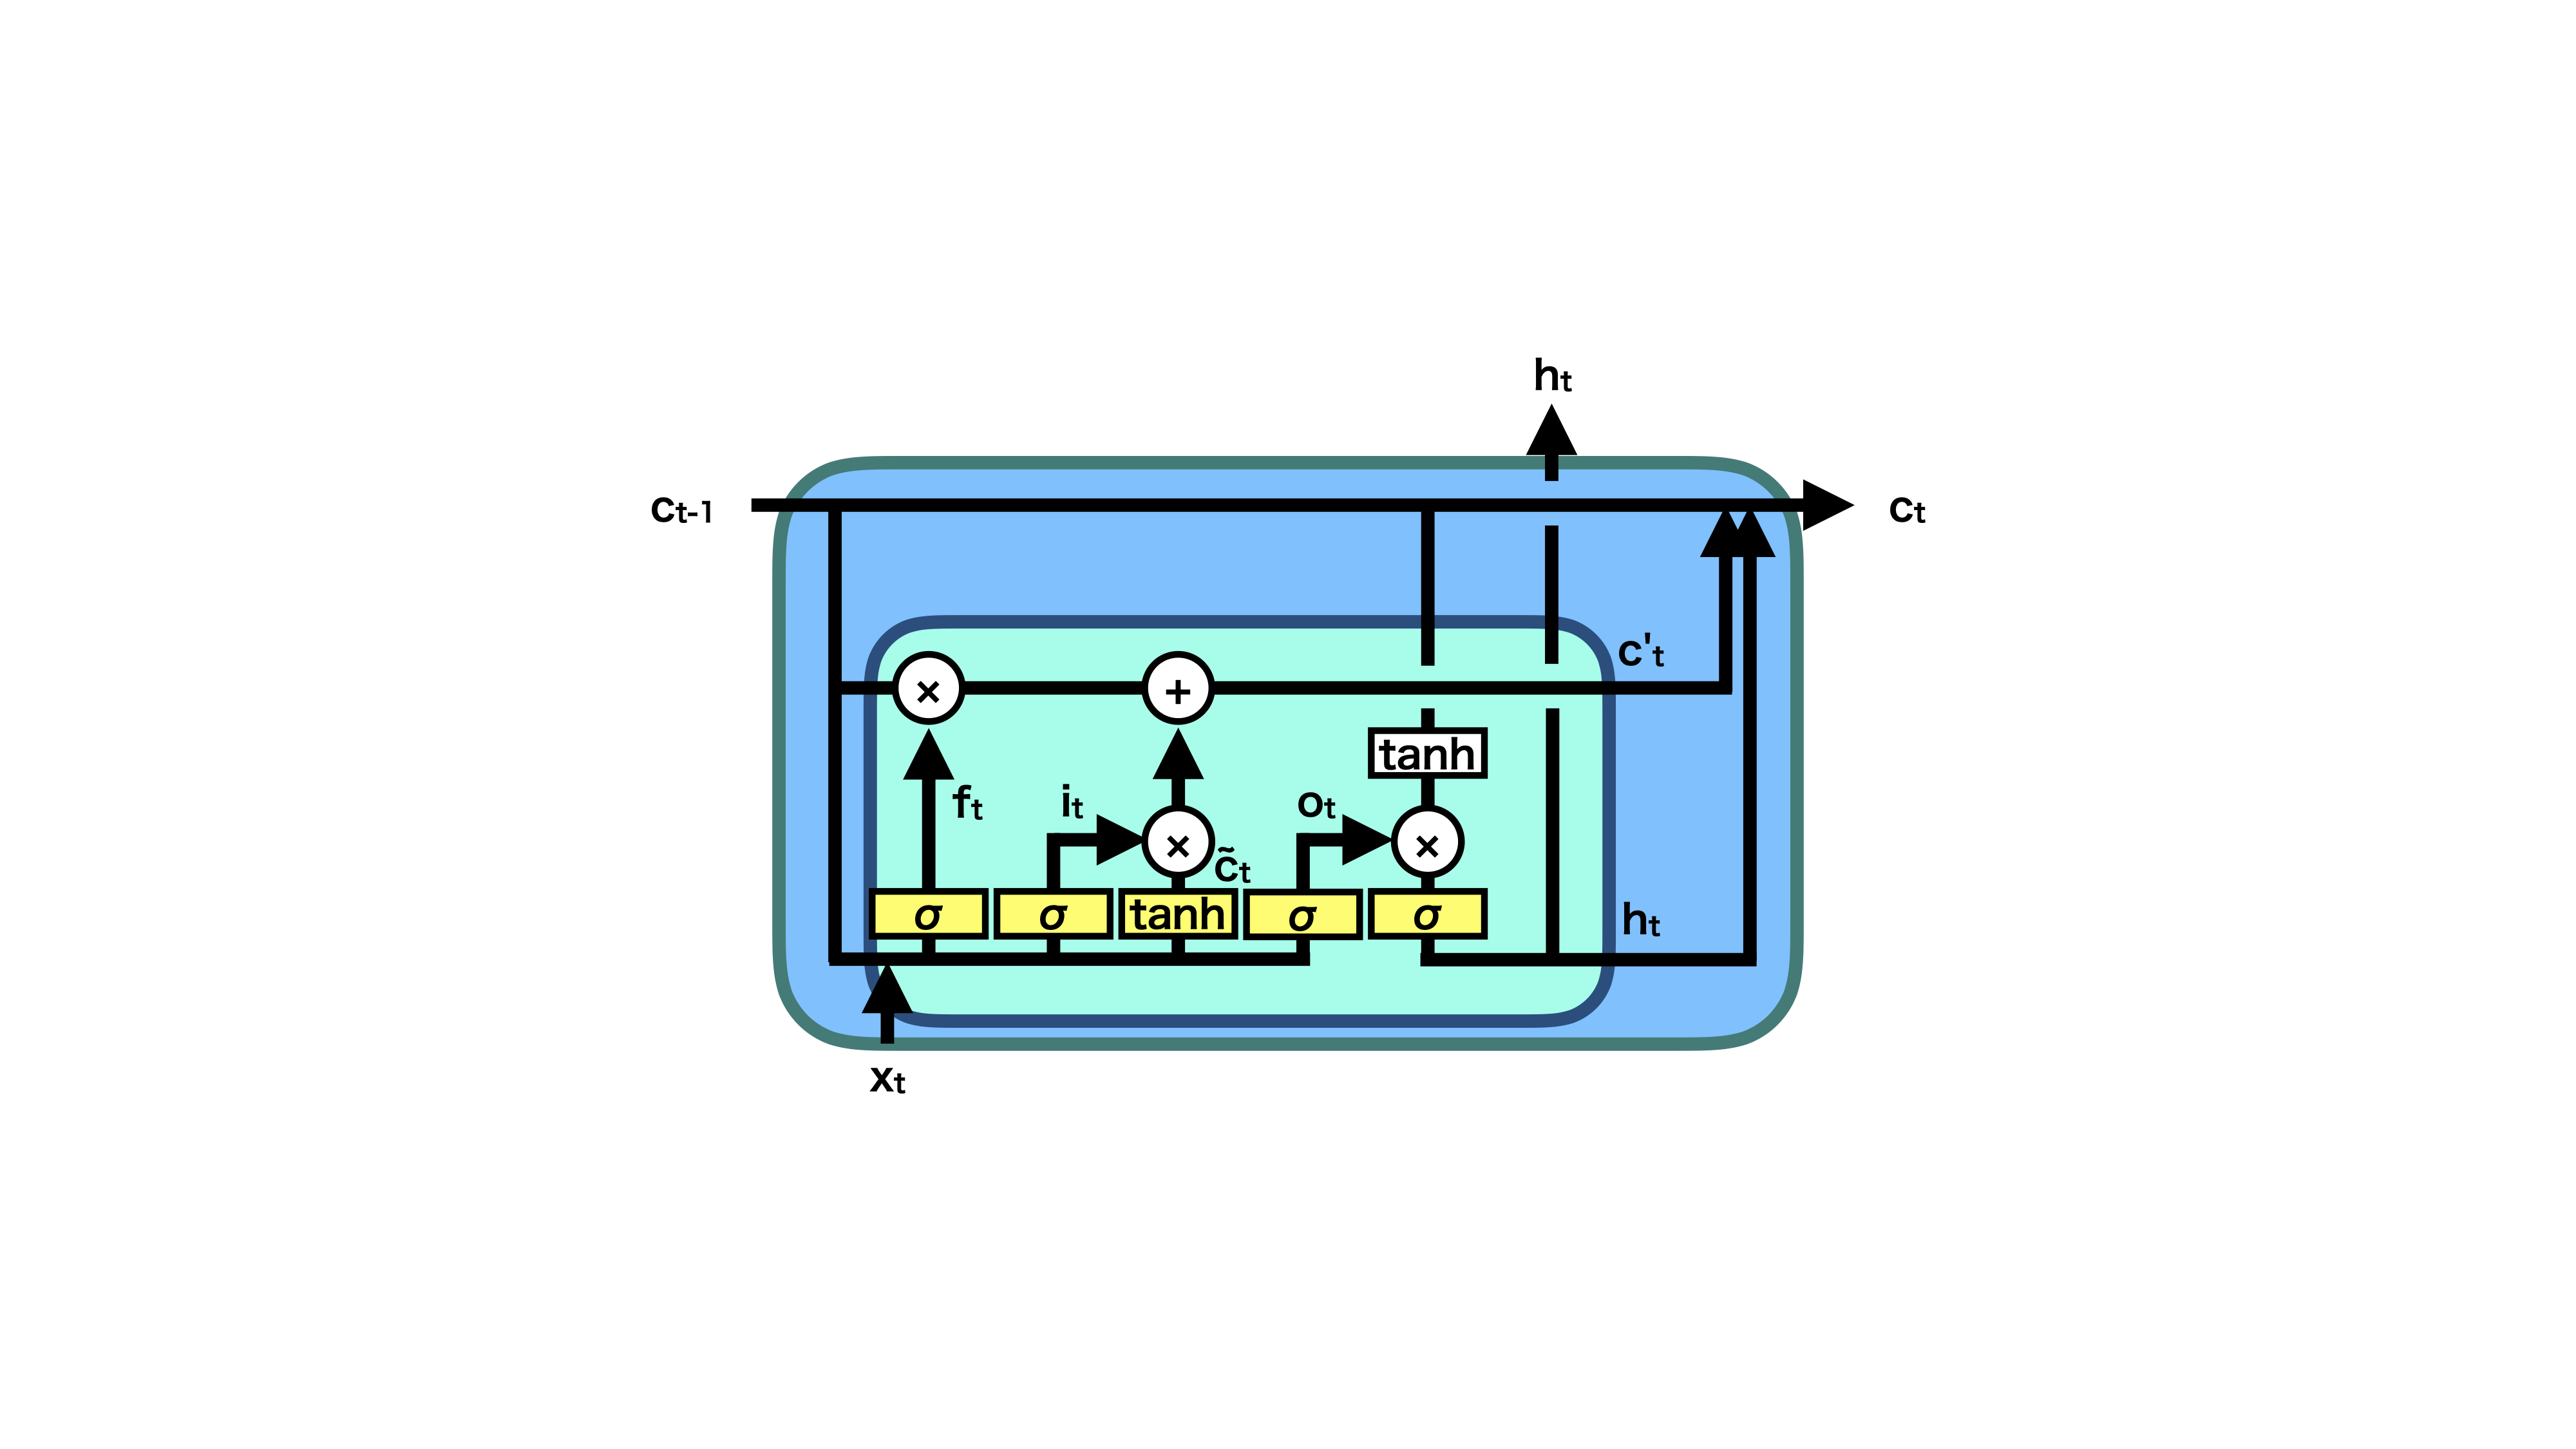
\includegraphics[width=0.9\textwidth]{Figure/3Networks/3-4-2-1VLSTMStructure.png}
 \caption{自作リカレントニューラルネットワークの構造}
 \label{3-4-2-1VLSTMStructure}
\end{figure}

\begin{figure}[h]
 \centering
 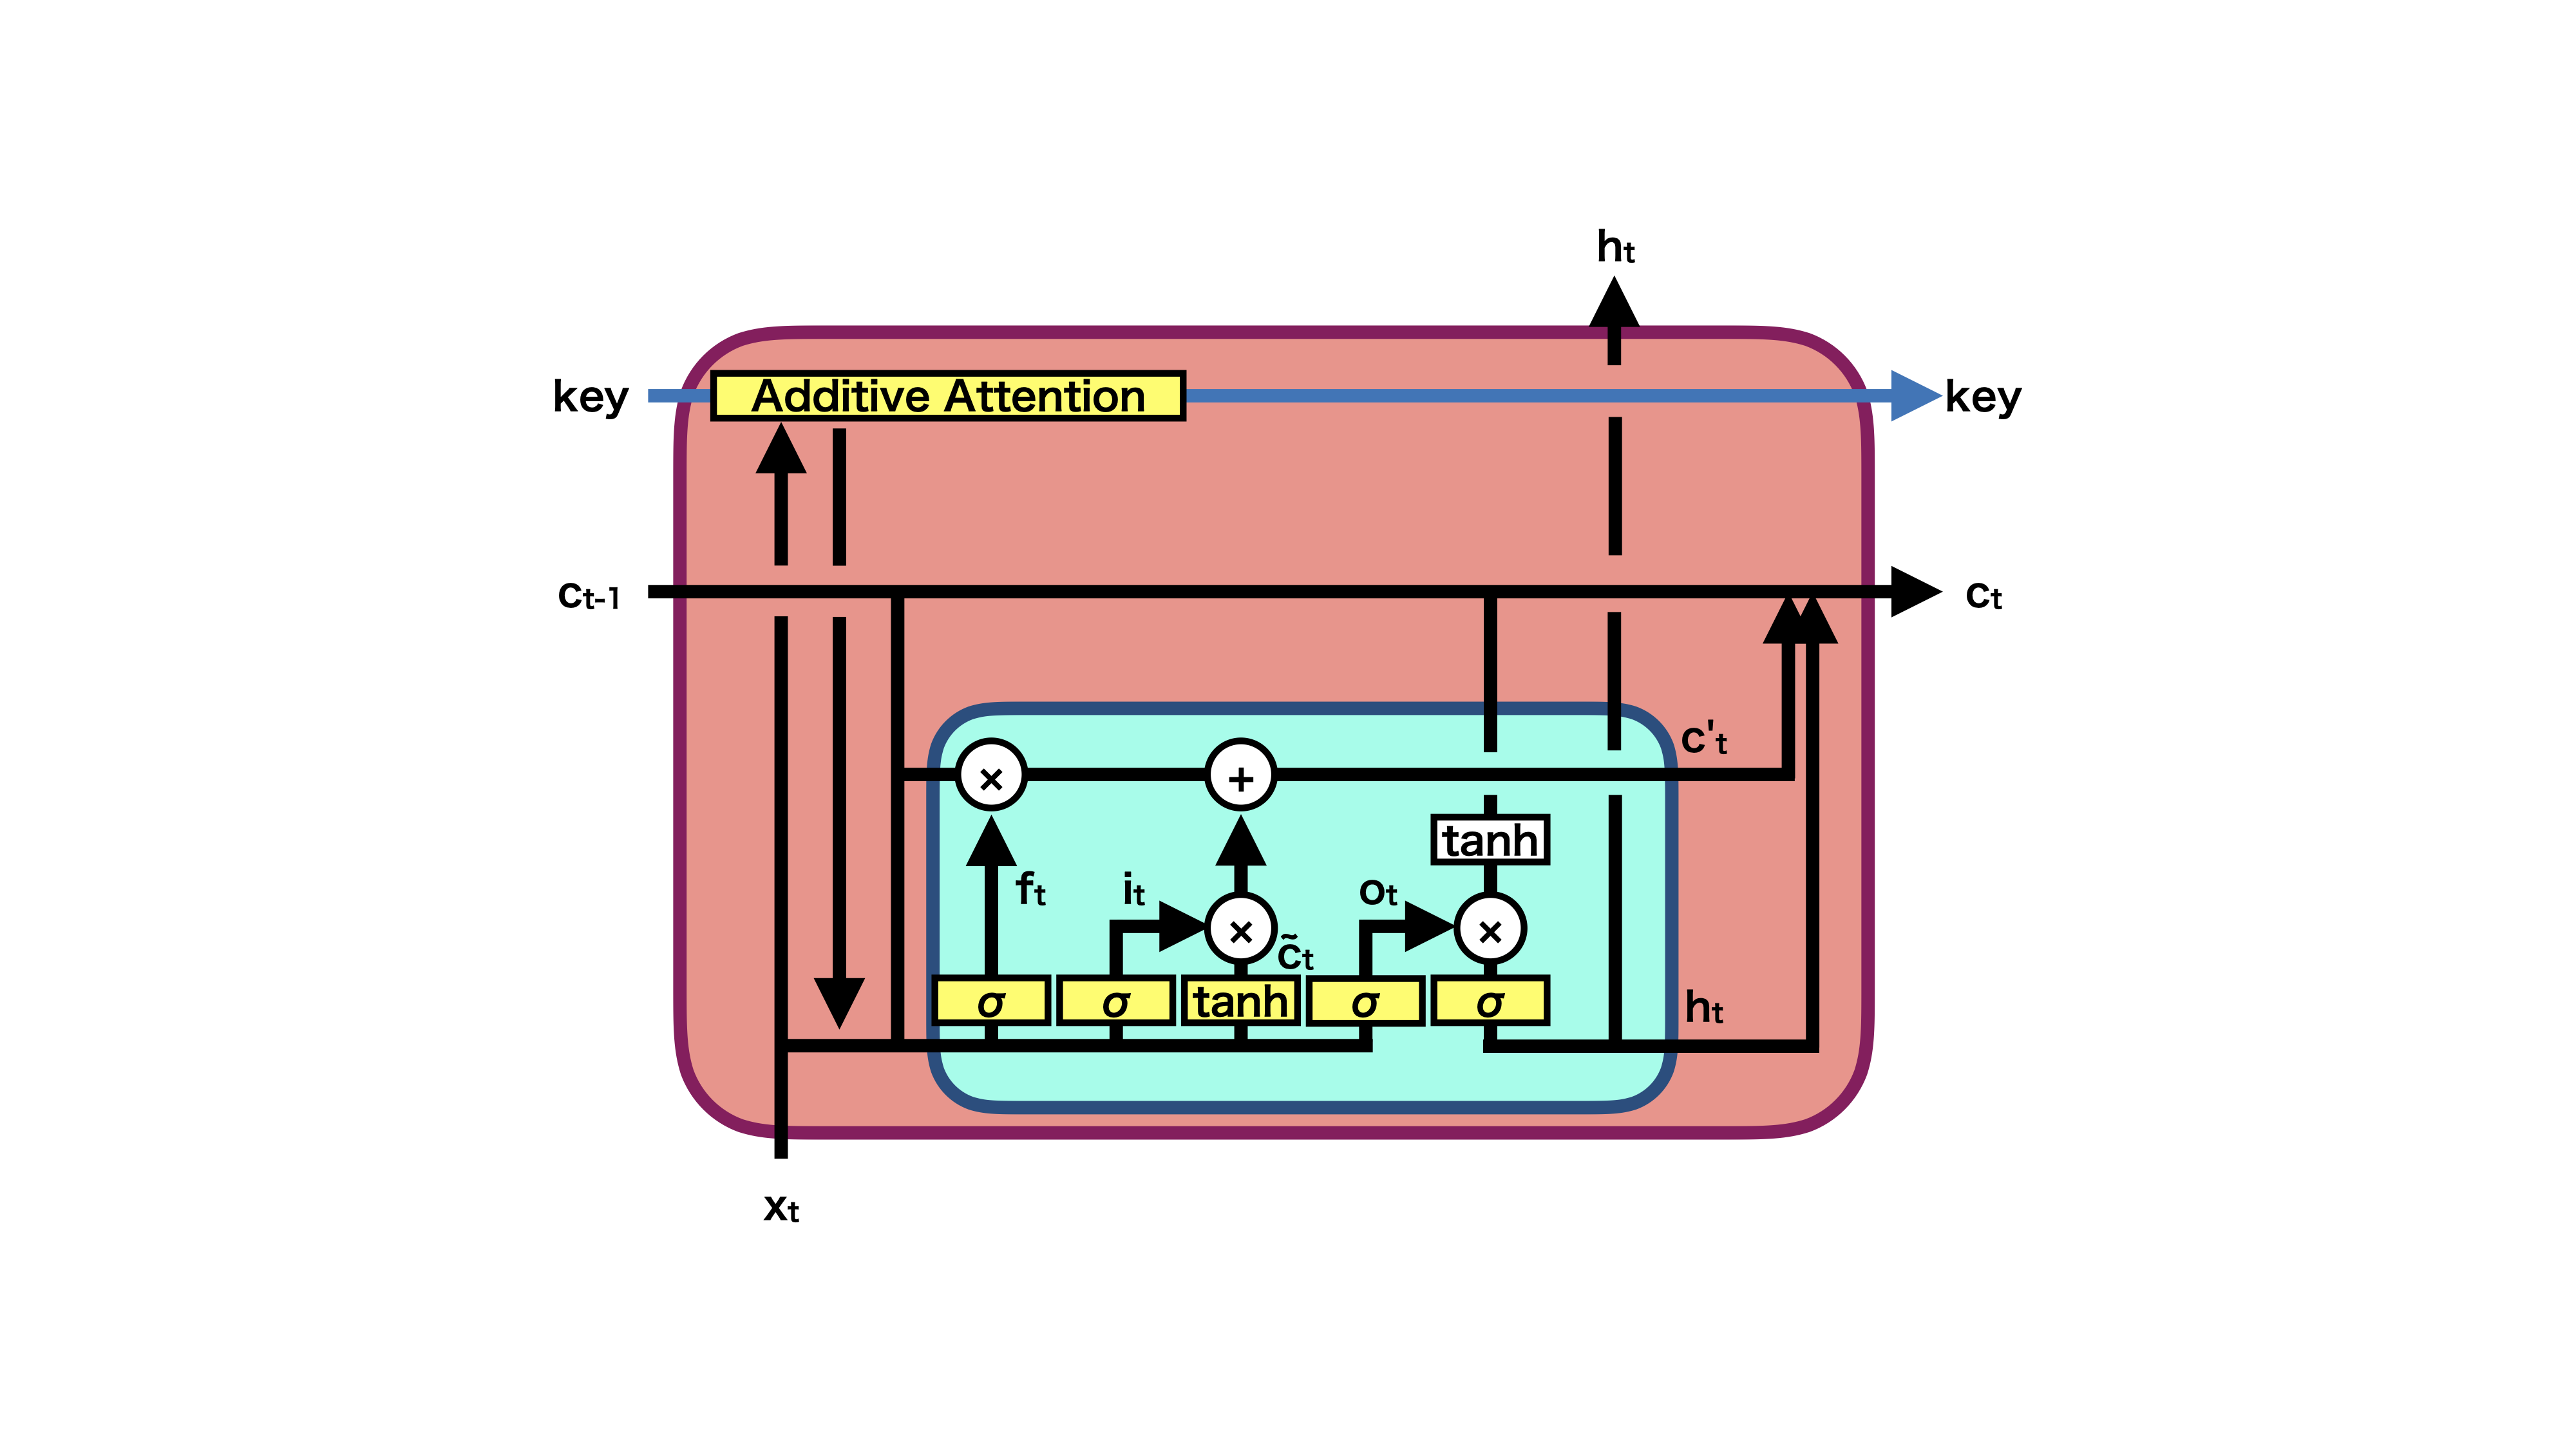
\includegraphics[width=0.9\textwidth]{Figure/3Networks/3-4-2-2AttentionVLSTM.png}
 \caption{Attentionを組み込んだ自作リカレントニューラルネットワークの構造}
 \label{3-4-2-2AttentionVLSTM}
\end{figure}


%%%%%%%%%%%%%%%%%%%%%%%%%%%%%%%%%%%%%%%%%%%%%%%%%%%%%%%%%%%%%%%%%%%%%%%%
\subsection{ネットワークの学習と戦略} \label{Net:VLSTM:TrainingandStrategyofVLSTM}

訓練データ\\
ゼロパディング

飛跡順のシャッフル

%%%%%%%%%%%%%%%%%%%%%%%%%%%%%%%%%%%%%%%%%%%%%%%%%%%%%%%%%%%%%%%%%%%%%%%%
\subsection{ネットワークの性能} \label{Net:VLSTM:PerformanceofVLSTM}

ハイパーパラメータ・チューニング\\

事象についての情報による変化\\

Attention weight\\

bb, ccデータセット









